\documentclass[11pt,a4paper,twoside]{tesis}
% SI NO PENSAS IMPRIMIRLO EN FORMATO LIBRO PODES USAR
%\documentclass[11pt,a4paper]{tesis}
\usepackage{tikz}
\usetikzlibrary{automata, positioning}
\usepackage{graphicx}
\usepackage[utf8]{inputenc}
\usepackage[spanish]{babel}
\usepackage{listings}
\usepackage[left=3cm,right=3cm,bottom=3.5cm,top=3.5cm]{geometry}


% Configuración del paquete de pseudocódigo
\lstset{
  basicstyle=\ttfamily\scriptsize,
  mathescape=true,
  captionpos=b,
  frame=single,
  keywordstyle={\color{BrickRed}},
  keywordstyle=[2]{\color{OliveGreen}},
  keywordstyle=[3]{\color{MidnightBlue}},
  commentstyle=\color{OliveGreen},
}

\lstdefinelanguage{pseudocode}{
  comment=[l]{//},
  morekeywords=[3]{if,then,else,for,while,do,return,procedure,function,such,that,let,true,false}
}
\lstset{escapeinside={(*@}{@*)}}
\lstset{numbers=left, numberstyle=\tiny, stepnumber=1, numbersep=8pt}


\usepackage{algorithm}
\usepackage{algpseudocode}
			% configure language options
\usepackage[utf8x]{inputenc}									% configure input encoding
\usepackage[inline]{enumitem}									% control layout of itemize, enumerate, description
\usepackage{xspace}	
\usepackage{multicol,lipsum}
% correct added/missing spaces made by tex decoder
\usepackage{pifont}												% for check and cross marks
\usepackage{mathtools}                                          % load amsmath, position eqs at fixed position,etc
\usepackage{amssymb}											% for extra symbols
%\usepackage{amsthm}											%for qed
\usepackage{trimclip}                                           % for cliping symbols in boxes
\usepackage[usenames,dvipsnames,svgnames,table]{xcolor}			% adds use of colors
\usepackage{listings}											% for the lstlisting environment
\usepackage{url}                                                % for url and hyperlinks
 \usepackage{ulem}   % for crossing out thinks.
        
\usepackage[hidelinks]{hyperref}

\usepackage[section]{placeins}

\usepackage{subfigure}
\usepackage{ifthen}
%%%%%%%%%%%%%%%%%%%%%%%%%%%%%%%%%%%%%%%%%%%%%%%%%%%%%%%%%%%%%%%%%%%%%%%%%%%%%%%
%%  Modifiers and Fonts
%%%%%%%%%%%%%%%%%%%%%%%%%%%%%%%%%%%%%%%%%%%%%%%%%%%%%%%%%%%%%%%%%%%%%%%%%%%%%%%

\renewcommand{\k}[1]{\textit{#1}}
\newcommand{\mk}[1]{\mathit{#1}}

\renewcommand{\v}[1]{\texttt{#1}}
\newcommand{\mv}[1]{\text{\small\textsf{#1}}\xspace}
\newcommand{\mvs}[1]{\text{\scriptsize\textsf{#1}}\xspace}

\newcommand{\sref}[2]{\ref{#1}{\color{BrickRed}.}{\subref*{#1:#2}}}

%%%%%%%%%%%%%%%%%%%%%%%%%%%%%%%%%%%%%%%%%%%%%%%%%%%%%%%%%%%%%%%%%%%%%%%%%%%%%%%
%%  Symbols
%%%%%%%%%%%%%%%%%%%%%%%%%%%%%%%%%%%%%%%%%%%%%%%%%%%%%%%%%%%%%%%%%%%%%%%%%%%%%%%

% Tildes and crosses

\newcommand{\Y}{\ding{51}}
\newcommand{\N}{\ding{55}}

% Math

\newcommand{\card}[1]{\lvert#1\rvert}
\newcommand{\<}{\langle}
\renewcommand{\>}{\rangle}
\newcommand{\ldot}{\;.\;}
\newcommand{\lcom}{\,,\,}
\newcommand{\primeI}[1]{{#1}'}
\newcommand{\primeII}[1]{{#1}'\!\!\:'}
\newcommand{\into}{\mapsto}
\newcommand{\Nat}{\mathbb{N}}
\newcommand{\dotrightarrow}{\clipbox{0pt 0 {.675\width} 
0}{\ensuremath{\rightarrow}} \makebox[1.1pt]{} {\cdot} {\cdot} {\cdot} 
\makebox[1.1pt]{} \clipbox{{.55\width} 0 0pt -1pt}{\ensuremath{\rightarrow}}}
\newcommand{\longdotrightarrow}{\clipbox{0pt 0 {.55\width} 
0}{\ensuremath{\rightarrow}} \makebox[2pt]{} {\cdot} \makebox[1pt]{} {\cdot} 
\makebox[1pt]{} {\cdot} \makebox[2pt]{} \clipbox{{.45\width} 0 0pt 
0}{\ensuremath{\rightarrow}}}

% Sets

\newcommand{\C}{\subseteq}
\newcommand{\x}{\times}

% Logic

\newcommand{\true}{\mk{true}}
\newcommand{\false}{\mk{false}}
\renewcommand{\iff}{\Leftrightarrow}
\newcommand{\then}{\Rightarrow}

% Tools

\newcommand{\MTSA}{{\scshape mtsa}\xspace}
\newcommand{\SUP}{{\scshape supremica}\xspace}
\newcommand{\MBP}{{\scshape mbp}\xspace}
\newcommand{\PRP}{{\scshape prp}\xspace}
\newcommand{\MYND}{{\scshape mynd}\xspace}
\newcommand{\RATSY}{{\scshape ratsy}\xspace}
\newcommand{\ACACIA}{{\scshape acacia+}\xspace}
\newcommand{\SLUGS}{{\scshape slugs}\xspace}
\newcommand{\CIRCA}{{\scshape circa}\xspace}
\newcommand{\PARTY}{{\scshape party}\xspace}
\newcommand{\GPT}{{\scshape gpt}\xspace}
\newcommand{\DCS}{{\scshape otf-dcs}\xspace}
\newcommand{\DCSRA}{{\scshape otf-dcs-ra}\xspace}
%\newcommand{\DCSRAMON}{{\scshape mon-dcs-ra}\xspace}
\newcommand{\DCSBFS}{{\scshape otf-dcs-bfs}\xspace}
\newcommand{\DCSMA}{{\scshape otf-dcs-ma}\xspace}

% Supervisory Control

\renewcommand{\l}{\ell}
\renewcommand{\ll}{{\bar{\l}}}
\renewcommand{\d}{\delta}
\newcommand{\init}[1]{\bar{#1}} % #1 state name
\newcommand{\state}[2]{{#1}^{#2}}
\newcommand{\s}[1]{\state{e}{#1}}

\newcommand{\D}{\rightarrow}
\newcommand{\B}{\rightsquigarrow}

\newcommand{\A}{\mathcal{A}}
\newcommand{\E}{\mathcal{E}}
\newcommand{\G}{\mathcal{G}}
\newcommand{\M}{\mathcal{M}}
\newcommand{\R}[2]{{#1 \mathrel{R} #2}}
\newcommand{\W}{\mathcal{W}}

\renewcommand{\L}{\mathcal{L}}
\renewcommand{\P}{\mathcal{P}}
\renewcommand{\S}{\mathcal{S}}

\newcommand{\w}{\ensuremath{\omega}}

% Entornos de teoremas/definiciones (Jansen et al. 2019), usados en el Cap. 3
\theoremstyle{definition}
\newtheorem{definition}{Definición}[section]
\theoremstyle{plain}
\newtheorem{theorem}[definition]{Teorema}
\newtheorem{lemma}[definition]{Lema}
\newtheorem{proposition}[definition]{Proposición}

% Notación de branching bisimilarity (Jansen et al. 2019), usada en el Cap. 3
\newlength{\leftrightarrowwidth}
\settowidth{\leftrightarrowwidth}{$\leftrightarrow$}
\newcommand{\bisauxiliary}{\raisebox{.3ex}{\makebox[\leftrightarrowwidth]{$\underline{\makebox[0.7\leftrightarrowwidth]{$\leftrightarrow$}}$}}}
\newcommand{\bbis}{\mathrel{\bisauxiliary_b\!}}
\newcommand{\pijl}[1]{\mathrel{\text{$\xrightarrow{\smash[t]{#1}}$}}}
\newcommand{\lijp}[1]{\mathrel{\text{$\xleftarrow{\smash[t]{#1}}$}}}
% Slices y conjuntos derivados de las particiones Pi_s y Pi_t (Cap. 4)
\newcommand{\TB}{T_{B\pijl{}}}
\newcommand{\TBp}{T'_{B\pijl{}}}
\newcommand{\TBaB}{T_{B\pijl{a} B'}}
\newcommand{\TaB}{T_{\pijl{a} B'}}
\newcommand{\BT}{B_{\pijl{T}}}
% Ojo: \# esta redefinido mas abajo como \rapprox (notacion de DCS), asi que
% el numeral hay que tomarlo de la fuente de texto con \symbol{35}.
\newcommand{\hash}{\mathord{\text{\symbol{35}}}}
\newcommand{\nraB}{\hash aB'}
\newcommand{\Bottom}{\mathit{Bottom}}
\newcommand{\splittableBlocks}{\mathit{splittableBlocks}}

\newcommand{\notstep}[2]{\overset{#1}{\not\D}_{#2}}
\newcommand{\step}[2]{\overset{#1}{\D}_{#2}}
\newcommand{\mstep}[2]{\overset{#1}{\twoheadrightarrow}_{#2}}
\newcommand{\lstep}[2]{\overset{#1}{\longrightarrow}_{#2}}
\newcommand{\walk}[2]{\overset{#1}{\Rightarrow}_{#2}}
\newcommand{\hop}[2]{\overset{#1}{\B}_{#2}}
\newcommand{\runw}[2]{\,\overset{#1}{\dotrightarrow}_{#2}\,}
\newcommand{\run}[3]{
\,\overset{#1\ldots#2}{\longdotrightarrow}_{#3}\,}
\newcommand{\runlst}[3]{
\overset{#1\quad#2}{\raisebox{.1pt}{-}{\,\cdot\cdot\cdot}\!\D}_{#3}}
\newcommand{\enabled}[2]{\step{}{#1}\!\!(#2)}
\newcommand{\runs}[2]{\runw{}{#1}\!\!(#2)}

\newcommand{\trimlst}[1]{\trimbox{0 0 0 5pt}{\ensuremath{#1}}}

% DCS

\newcommand{\ma}[1]{\tilde{#1}}
\renewcommand{\#}{\text{\rapprox}}
\newcommand{\rapprox}{\protect\raisebox{.09em}{\:\!\protect\reflectbox{\protect\rotatebox[origin=c]{90}{\ensuremath{\approx}}}}}

\newcommand{\dist}[1]{\makebox[6pt][c]{\raisebox{0pt}[6pt][1.5pt]{\ensuremath{\scriptscriptstyle #1}}}}

\newcommand{\CCC}{\mathbb{C}}
\newcommand{\WCCC}{\mathbb{W}}

\newcommand{\open}{\mk{open}}
\newcommand{\recommendations}{\mk{RT}} %{\mathcal{R}} %\mk{recommendations}
\newcommand{\Goals}{\mk{Goals}}
\newcommand{\Errors}{\mk{Errors}}
\newcommand{\Witness}{\mk{Witnesses}}
\newcommand{\NONE}{\mk{None}}
\newcommand{\Unsettled}{\mk{Unsettled}}

%nuevos:  ------------------------------------------------------------
\newcommand{\pathBetween}[2]{(#1 \step{\l}{E} #2\runw{}{\structure} #1)}

\newcommand{\unexploredToBottom}[1]{\mk{#1_{\bot}}}
\newcommand{\unexploredToTop}[1]{\mk{#1_{\top}}}


%\newcommand{\unexploredToBottom}[1]{\mk{#1_{?\rightarrow \bot}}}
%\newcommand{\unexploredToTop}[1]{\mk{#1_{?\rightarrow \top}}}

\newcommand{\forcedTo}[3]{\mk{(#1\twoheadrightarrow #2)_{#3}}}

\newcommand{\WES}{\mk{W_{\unexploredToBottom{\structure}}}}
\newcommand{\WESS}{\mk{W_{\unexploredToBottom{\structure'}}}}
\newcommand{\LES}{\mk{L_{\unexploredToTop{\structure}}}}
\newcommand{\LESS}{\mk{L_{\unexploredToTop{\structure'}}}}
\newcommand{\WE}{\mk{W_E}}
\newcommand{\LE}{\mk{L_E}}

\newcommand{\SCC}{\mk{loops}} %strongly connected component

\newcommand{\Loops}[2]{AllNoneLoops(#1,#2)}

%\newcommand{\controllerReachsGoalsInOneStep}[1]{\mk{(\exists \l \ldot \trimlst{#1 \step{\l}{E} e''} \wedge e'' \in \Goals)    \wedge (\forall \l_u \in A_E^U \ldot \trimlst{#1 \step{\l_u}{E} e''} \then e'' \in \Goals)}}


\newcommand{\marked}[2]{\mk{\exists e_m \in #1 \ldot e_m \in M_{#2}}}
\newcommand{\Marked}{\mathit{Marked}}
\newtheorem{invariante}[definition]{Invariante}

\newcommand{\descendants}{\mk{descendants}}

\newcommand{\Targets}{Targets\newcommand{\Targets}{Targets}

}
%----------------------------------------------------------------------

\newcommand{\heuristic}{\mk{heuristic}}
\newcommand{\initial}{\ensuremath{\init{e}}}
\newcommand{\current}{\ensuremath{s}}
\newcommand{\child}{\ensuremath{s'}}
\newcommand{\structure}{\mk{ES}}
\newcommand{\toOpen}{\mk{toOpen}}

\newcommand{\ancestors}{\mk{ancestors}}
\newcommand{\predecesor}{\mk{predecesor}}
\newcommand{\statusu}{\mk{status}}
\newcommand{\visited}{\mk{visited}}
\newcommand{\pending}{\mk{pending}}
\newcommand{\unconfirmed}{\mk{unconfirmed}}

\newcommand{\target}{\mk{target}}
\newcommand{\novel}{\mk{novel}}
\newcommand{\distant}{\mk{distant}}
\newcommand{\strides}{\mk{strides}}

\newcommand{\MA}[2]{\mk{MA}_{#1}^{#2}}
\newcommand{\RA}[2]{\mk{RA}_{#1}^{#2}}

\newcommand{\g}{\ensuremath{g}}
\newcommand{\m}{m}%{\mathsf{m}}
\newcommand{\rr}{r}%{\mathsf{r}}
\newcommand{\pp}{p}%{\mathsf{p}}





\newboolean{showcomments}
\setboolean{showcomments}{true} % comment this line to 
%deactivate comments


% author macros ------------------------------------------------------------
\ifthenelse{\boolean{showcomments}}
{
	\newcommand{\ugh}[1]{\textcolor{red}{\uwave{#1}}}   
	% please rephrase
	\newcommand{\ins}[1]{\textcolor{blue}{\uline{#1}}}  % 
	%please insert
	\newcommand{\del}[1]{\textcolor{red}{\sout{#1}}}    % 
	%please delete
	\newcommand{\chg}[2]{
		\textcolor{red}{\sout{#1}}{$\rightarrow$}
		\textcolor{blue}{\uline{#2}}}               % please change
}{
	\newcommand{\ugh}[1]{#1}                            % please 
	%rephrase
	\newcommand{\ins}[1]{#1}                            % please insert
	\newcommand{\del}[1]{}                              % please delete
	\newcommand{\chg}[2]{#2}
}

\ifthenelse{\boolean{showcomments}}{
	\newcommand{\nbc}[3]{
		{\colorbox{#3}{\bfseries\sffamily\scriptsize\textcolor{white}{#1}}}
		{\textcolor{#3}{\sf\small$\langle$\textit{#2}$\rangle$}}}
}{
	\newcommand{\nbc}[3]{}
	\newcommand{\version}{}
}

\newcommand\su[1]{\nbc{SU}{#1}{red}} 
\newcommand\cl[1]{\nbc{CL}{#1}{pink}} 
\newcommand\hg[1]{\nbc{HG}{#1}{olive}}
\newcommand\vb[1]{\nbc{VB}{#1}{teal}}

\newcommand\resolved[1]{}
% add more author macros here

\newcommand\tocado[1]{\textcolor{red}{#1}}
\newcommand\comment[1]{\textcolor{cyan}{#1}}

\newcommand{\multlinecomment}[1]{\directlua{-- #1}}

\newcommand{\Review}[1]{#1}

%%%%%%%%%%%%%%%%%%%%%%%%%%%%%%%%%%%%%%%%%%%%%%%%%%%%%%%%%%%%%%%%%%%%%%%%%%%%%%%
%%  Notacion de complejidad y llaves de costo en los algoritmos (Cap. 4)
%%  Tomados de las fuentes de Jansen et al. (arXiv:1909.10824).
%%%%%%%%%%%%%%%%%%%%%%%%%%%%%%%%%%%%%%%%%%%%%%%%%%%%%%%%%%%%%%%%%%%%%%%%%%%%%%%

\newcommand{\bigo}[1]{{O\!\left(#1\right)}}
\newcommand{\bigO}{O}                                   % O sin argumento
\newcommand{\size}[1]{\left\lvert #1 \right\rvert}

% \rightbrace{<lineas>}{<texto>}: llave gris al margen derecho de un bloque de
% pseudocodigo, para anotar su costo.
\newlength{\halflineskip}
\newcommand{\rightbrace}[3][0]{\setlength{\halflineskip}{0.5\baselineskip}\hspace{0pt plus 1filll}\makebox[0pt][l]{\smash{\tikz[baseline=#1\baselineskip]{\draw[thick,color=gray,line cap=round,decorate,decoration={brace,amplitude=2.3pt}] (0pt,0.7\baselineskip) ++(0.1em,0) -- ++(0pt,-#2\baselineskip+1pt) (5pt,\halflineskip-#2\halflineskip) node[color=gray,right,inner sep=0.1em,anchor=base west]{\small #3};}}}}

% Comentarios en gris dentro de los algoritmos
\renewcommand{\algorithmiccomment}[1]{\hfill{\color{gray}// #1}}

% Rotulo del float de algoritmos ("Algorithm 1" -> "Algoritmo 1")
\makeatletter
\renewcommand{\ALG@name}{Algoritmo}
\makeatother
\renewcommand{\listalgorithmname}{Índice de algoritmos}

% Palabras clave del pseudocodigo en castellano. Las compuestas
% (\algorithmicendif, \algorithmicendfor, \algorithmicendwhile, ...) se derivan
% de \algorithmicend y de la palabra correspondiente, asi que salen solas.
\renewcommand{\algorithmicrequire}{\textbf{Requiere:}}
\renewcommand{\algorithmicensure}{\textbf{Asegura:}}
\renewcommand{\algorithmicend}{\textbf{fin}}
\renewcommand{\algorithmicif}{\textbf{si}}
\renewcommand{\algorithmicthen}{\textbf{entonces}}
\renewcommand{\algorithmicelse}{\textbf{si no}}
\renewcommand{\algorithmicelsif}{\textbf{si no, si}}
\renewcommand{\algorithmicfor}{\textbf{para}}
\renewcommand{\algorithmicforall}{\textbf{para todo}}
\renewcommand{\algorithmicdo}{\textbf{hacer}}
\renewcommand{\algorithmicwhile}{\textbf{mientras}}
\renewcommand{\algorithmicloop}{\textbf{repetir}}
\renewcommand{\algorithmicrepeat}{\textbf{repetir}}
\renewcommand{\algorithmicuntil}{\textbf{hasta que}}
\renewcommand{\algorithmicprint}{\textbf{imprimir}}
\renewcommand{\algorithmicreturn}{\textbf{retornar}}
\renewcommand{\algorithmicand}{\textbf{y}}
\renewcommand{\algorithmicor}{\textbf{o}}
\renewcommand{\algorithmicnot}{\textbf{no}}
\renewcommand{\algorithmicto}{\textbf{hasta}}
\renewcommand{\algorithmicinputs}{\textbf{entradas}}
\renewcommand{\algorithmicoutputs}{\textbf{salidas}}
\renewcommand{\algorithmicglobals}{\textbf{globales}}
\renewcommand{\algorithmicbody}{\textbf{hacer}}
\renewcommand{\algorithmictrue}{\textbf{verdadero}}
\renewcommand{\algorithmicfalse}{\textbf{falso}}

%%%%%%%%%%%%%%%%%%%%%%%%%%%%%%%%%%%%%%%%%%%%%%%%%%%%%%%%%%%%%%%%%%%%%%%%%%%%%%%
%%  Estilos tikz para las figuras de bloques y bunches (Cap. 4)
%%  Tomados de las fuentes de Jansen et al. (arXiv:1909.10824).
%%  Van agrupados en el estilo `bunchpic' para que la redefinicion de `state'
%%  quede local a cada tikzpicture y no afecte a los automatas de los otros
%%  capitulos (que usan el `state' de la libreria automata).
%%%%%%%%%%%%%%%%%%%%%%%%%%%%%%%%%%%%%%%%%%%%%%%%%%%%%%%%%%%%%%%%%%%%%%%%%%%%%%%

\newlength{\statetextwidth}\settowidth{\statetextwidth}{$s_0$}
\newlength{\statetextheight}\settoheight{\statetextheight}{$s_0$}
\newlength{\statetextdepth}\settodepth{\statetextdepth}{$s_0$}

\tikzset{bunchpic/.style={
	bunch/.style={very thin,draw,fill=gray!5},
	block/.style={thick,draw,fill=gray!15,rounded corners=4.95mm},
	state/.style={circle,draw,semithick,fill=white,inner sep=1.35pt,
		text height=\statetextheight,text depth=\statetextdepth},
	% Estados rayados: verticales para los destinados a R, horizontales para
	% los destinados a U. Se usan rayas (y no solo color) para que las figuras
	% se sigan entendiendo impresas en blanco y negro.
	red state/.style={state,fill=red!10,path picture={\draw[red!40,very thick]
		(-0.25\statetextwidth,-1cm) -- (-0.25\statetextwidth,2cm)
		(0cm,-1cm) -- (0cm,2cm)
		(0.25\statetextwidth,-1cm) -- (0.25\statetextwidth,2cm)
		(0.5\statetextwidth,-1cm) -- (0.5\statetextwidth,2cm)
		(0.75\statetextwidth,-1cm) -- (0.75\statetextwidth,2cm)
		(\statetextwidth,-1cm) -- (\statetextwidth,2cm)
		(1.25\statetextwidth,-1cm) -- (1.25\statetextwidth,2cm);}},
	blue state/.style={state,fill=blue!10,path picture={\draw[blue!40,very thick]
		(-1cm,0.5\statetextheight-0.5\statetextdepth+0.75\statetextwidth) -- (2cm,0.5\statetextheight-0.5\statetextdepth+0.75\statetextwidth)
		(-1cm,0.5\statetextheight-0.5\statetextdepth+0.5\statetextwidth) -- (2cm,0.5\statetextheight-0.5\statetextdepth+0.5\statetextwidth)
		(-1cm,0.5\statetextheight-0.5\statetextdepth+0.25\statetextwidth) -- (2cm,0.5\statetextheight-0.5\statetextdepth+0.25\statetextwidth)
		(-1cm,0.5\statetextheight-0.5\statetextdepth) -- (2cm,0.5\statetextheight-0.5\statetextdepth)
		(-1cm,0.5\statetextheight-0.5\statetextdepth-0.25\statetextwidth) -- (2cm,0.5\statetextheight-0.5\statetextdepth-0.25\statetextwidth)
		(-1cm,0.5\statetextheight-0.5\statetextdepth-0.5\statetextwidth) -- (2cm,0.5\statetextheight-0.5\statetextdepth-0.5\statetextwidth)
		(-1cm,0.5\statetextheight-0.5\statetextdepth-0.75\statetextwidth) -- (2cm,0.5\statetextheight-0.5\statetextdepth-0.75\statetextwidth);}}
}}

%%  Marcas en linea para referirse a los estados rayados desde el texto.
\newcommand{\redstatetext}{\smash{\tikz[bunchpic,baseline=-0.37\statetextwidth]{%
	\node[red state,thin,inner sep=0pt]{\makebox[0.5\statetextwidth]{}};}}}
\newcommand{\bluestatetext}{\smash{\tikz[bunchpic,baseline=-0.37\statetextwidth]{%
	\node[blue state,thin,inner sep=0pt]{\makebox[0.5\statetextwidth]{}};}}}


\begin{document}

%%%% CARATULA

\def\autor{Hernán Gabriel Gagliardi}
\def\tituloTesis{Definición y análisis de etapas de exploración on-the-fly para síntesis de controladores del tipo non-blocking}
\def\runtitulo{Definición y análisis de etapas de exploración on-the-fly para síntesis de controladores del tipo non-blocking}
\def\runtitle{Star Wars: Rebellion and Empire}
\def\director{Sebastian Uchitel}
\def\codirector{Sebastian Zudaire}
\def\lugar{Buenos Aires, 2024}
\input{caratula}

%%%% ABSTRACTS, AGRADECIMIENTOS Y DEDICATORIA
\frontmatter
\pagestyle{empty}
%\begin{center}
%\large \bf \runtitulo
%\end{center}
%\vspace{1cm}
\chapter*{\runtitulo}

\noindent Esta tesis presenta la definición y análisis exploratorio sobre las fases que están involucradas en el algoritmo \textit{on-the-fly} de síntesis de directores para resolver problemas de Control de Eventos Discretos con la propiedad central de tipo non-blocking. Se busca de esta manera encontrar posibilidades de mejora en la heurística RA, la cual logra actualmente buenos resultados frente a heurísticas tradicionales.
Luego de realizada la exploración y análisis inicial sobre el comportamiento de las etapas en la exploración, implementamos algunos cambios sobre la
heurística RA para poder experimentar y analizar los resultados. De esa manera realizamos una propuesta de mejora para fortalecer las etapas de exploración analizadas previamente y lograr mejor \textit{performance}.
\bigskip

\noindent\textbf{Palabras claves:} Sistemas de Eventos Discretos, Síntesis de Controladores, Control Di- rigido, Control Supervisado, Síntesis on-the-fly, LTS, Non-Blocking.



\cleardoublepage
%%\begin{center}
%\large \bf \runtitle
%\end{center}
%\vspace{1cm}
\chapter*{\runtitle}

\noindent Compositional controller synthesis avoids state explosion by solving the problem piecewise: at each iteration it composes a subset of the plant, synthesises a partial controller, hides the local events and \textit{minimises} the result before returning it to the system. That minimisation step is what keeps the intermediate models from growing back, and it is also what dominates the cost of the method: it is solved by computing \textit{Weak Synthesis Observational Equivalence} (WSOE) with an $O(nm)$ algorithm.

\noindent In this thesis we propose replacing WSOE with \textit{branching bisimilarity}, for which an $O(m \log n)$ algorithm is available. We show that the replacement is not straightforward: under the natural hypothesis of hiding every local action, branching merges states that WSOE keeps apart, which would amount to over-reducing the model. We prove that restricting the internal actions to the \textit{uncontrollable} local ones yields $\sim_{B} \subseteq \sim_{W}$, and that the inclusion is strict. On that basis we implement the algorithm inside MTSA and integrate it into the compositional flow.

\noindent The evaluation was carried out on 2212 real minimisation instances captured from the synthesis flow itself. Correctness was validated against the reference implementation in mCRL2 and against the output of WSOE. As for performance, the final implementation stays below 1000~ms on the largest instances, where WSOE reaches 7600~ms, and in 83\% of the cases both equivalences produce the same reduction. The cost of the change shows up in memory usage.

\bigskip

\noindent\textbf{Keywords:} Discrete Event Systems, Controller Synthesis, Compositional Synthesis, Minimisation, Branching Bisimilarity, WSOE, Partition Refinement, LTS.
 % OPCIONAL: comentar si no se quiere

\cleardoublepage
\chapter*{Agradecimientos}

\noindent A Silvana y Beto, por criarme y acompañarme en cada paso con infinito amor. \\
\noindent A Mariana, Laura, Cecilia y Mariano, porque siempre me hicieron sentir querido, protegido y ayudado.
\\
\noindent A la casa de Perón, porque en comunidad transcurrió gran parte de la carrera y en donde Milagros, Ale, Julls, Alicia, Franco, Tito, Martín, Cabeza y Virginia me bancaron las jornadas de estudio y siguieron cada uno de mis exámenes.
\\
\noindent A Fernando, Pablo, Santiago y Juan Pablo por el ejercicio incesante de la amistad y por ser un ejemplo a seguir dentro y fuera de la facultad.
\\
\noindent A Fabio y a Roni, porque hicimos codo a codo cada examen, final y TP de la carrera.
\\
\noindent A Daniela, que en muchos momentos difíciles de la carrera supo ayudarme y convencerme de seguir.
\\
\\
\noindent Al Departamento de Computación y toda la gente que lo compone por ser una segunda casa desde hace tantos años. Al LaFHIS y todxs sus integrantes por haberme recibido en este último tramo con los brazos abiertos y haberme apoyado en todo momento.
\\
\noindent A mi director de Tesis Sebastian Uchitel y a mi co-director Sebastian Zudaire por la guía y por la inmensa generosidad con la que me acompañaron a lo largo de este trabajo.
\\
\\
\noindent A la militancia de Identidad, porque aprender de ellxs que vale la pena organizarse, luchar y trabajar por una facultad y un país mejor es una de las cosas más valiosas que me dejaron estos años. A Juliana y Abril, que me permiten irme del claustro con el inmenso orgullo de haber votado y acompañado a las primeras dos Presidentas Peronistas del CECEN.
\\
\\
\noindent A Julia porque construimos juntxs, desde el amor, los días más felices. % OPCIONAL: comentar si no se quiere

% \cleardoublepage
% \input{dedicatoria.tex}  % OPCIONAL: comentar si no se quiere

\cleardoublepage
\tableofcontents

\mainmatter
\pagestyle{headings}

%%%% ACA VA EL CONTENIDO DE LA TESIS
%% Capítulo 1
\chapter{Introducción}

% =====================================================================
% ESTRUCTURA OBJETIVO DE LA INTRODUCCIÓN (tema NUEVO de la tesis).
% NO BORRAR lo de abajo: gran parte del arranque sobre síntesis de
% controladores se reusa casi tal cual. Lo que hay que reescribir es el
% giro hacia "on-the-fly / heurística RA" (tema de la tesis-molde) y la
% guía de lectura, que apuntan a los capítulos viejos.
%
% Orden buscado:
%   1) Síntesis automática de controladores y por qué importa.   [REUSABLE: párrafos siguientes]
%   2) Composicionalidad: por qué se minimiza entre composiciones. [parte reusable, ver línea ~34]
%   3) El cuello de botella: WSOE en el paper composicional.       [FALTA -> \cite{compositional}]
%   4) Propuesta: reemplazar WSOE por branching bisimilarity con
%      el algoritmo eficiente de Groote et al. (2019).            [FALTA -> \cite{groote2019}]
%   5) Aportes y guía de lectura (a la estructura NUEVA: caps 2-7).[REESCRIBIR guía de lectura]
% =====================================================================

% \section{Introducción}
{\begin{small}%
\begin{flushright}%
\it

Lo que vieron mis ojos fue simultáneo: \\
lo que transcribiré, sucesivo, \\
porque el lenguaje lo es. \\
Algo, sin embargo, recogeré.

--JLB
\end{flushright}%
\end{small}%
\vspace{.5cm}}

La automatización de tareas ha sido a lo largo de la historia un desafío \textit{motivante} para las Ciencias de la Computación. Desde sus inicios se buscó la manera de automatizar las tareas tediosas o repetitivas. Yendo un poco más lejos, la posibilidad de una computadora que \textit{se programe} a sí misma es abordada por distintas ramas de la computación. Entre ellas se encuentran muchas agrupadas dentro del término \textit{Inteligencia Artificial}. En el trabajo que presentamos nos abocaremos al caso particular de programas que generan \textbf{Síntesis Automática de Controladores}.

En este área de estudio buscamos desarrollar código que \textbf{sintetice} una solución de un determinado problema de forma \textbf{automática} partiendo de ciertas \textit{reglas y objetivos} (o pre/post condiciones) que se proveen y es necesario cumplirlos. De esta manera, lo que devuelve nuestro programa es una estrategia que garantiza alcanzar una solución, si es que existe. Por otro lado, en el caso de que dadas las reglas y los objetivos planteados no exista una solución posible, avisa sobre la inexistencia de la misma. En el caso de garantizar la existencia de una solución, a la estrategia que permite alcanzarla se la conoce con el nombre de \textbf{Controlador}.

Este tipo de programas tienen múltiples aplicaciones, entre ellas podemos nombrar el control de aviones para demarcar incendios forestales \cite{ZudaireIncendio}, donde a veces incluso es necesario que el programa pueda adaptarse en medio de su ejecución.

El problema de \textit{síntesis} fue estudiado dentro de distintas áreas como: Control de Eventos Discretos \cite{DEC}, Síntesis Reactiva \cite{sreac} y Planning automático \cite{paut}. Si bien este trabajo se basa en resultados que provienen de combinar enfoques de las tres áreas, nos basamos principalmente en Control de Eventos Discretos (Discrete Event Control o DEC).

En este enfoque modelamos el problema utilizando autómatas finitos, también conocidos como máquinas de estados finitas. Un autómata finito, está conformado por estados y transiciones entre ellos. Podemos pensar los \textit{estados} como puntos y las transiciones como flechas de un solo sentido que unen a uno o varios de ellos. A estos puntos los llamamos estados ya que representan un momento particular del dominio que se quiere modelar, por ejemplo en el caso del avión mencionado anteriormente se podría hablar de estados que representen posibilidades como: \textit{avión aterrizado}, \textit{avión sin combustible}, \textit{avión en vuelo}, etc.

Por otro lado, vamos a tomar dentro de nuestro modelo a las transiciones como posibles acciones. En este caso algunas transiciones las podemos controlar y otras estarán fuera de nuestro alcance. Volviendo al ejemplo del avión, una acción \textbf{controlable} podría ser \textit{encendido de motor} mientras que la acción \textit{aterrizaje de emergencia} probablemente sea representada en nuestro modelo como una acción \textbf{no controlable}.

En el autómata mencionado además existen estados distinguidos. Por un lado tomaremos un estado como \textit{inicial} y será el estado desde el cual empezaremos la exploración. Además habrá \textit{estados objetivos} que serán los estados a los cuales buscaremos llegar. En este caso de análisis y a lo largo de la tesis llamaremos \textit{marcados} a estos estados objetivo y buscaremos que el sistema no solo pueda
alcanzarlos, sino que sea capaz de hacerlo infinitas veces y de manera segura. Esta última condición de \textit{seguridad} se refiere intuitivamente a que debemos llegar a un estado marcado mediante una secuencia de acciones que evite estados no controlables no deseados en el sistema. A esto se le agrega la condición de llegar al estado marcado infinitas veces, lo que refiere a que buscaremos poder mantenernos \textit{de forma controlable} con transiciones que nos garanticen un ciclo de permanencia en el estado marcado.

El valor de este enfoque y de un algoritmo que permita realizar síntesis es la generalización a distintos problemas. El autómata descripto puede modelar un avión como el caso mencionado, o el funcionamiento de una agencia de viajes como se verá en otro ejemplo o podrá modelar el funcionamiento de diversos problemas complejos. De todas formas, nuestro algoritmo podrá generar un \textbf{controlador} sin necesitar ningún cambio específico. Para lograr esto trabajará un experto en el área, quien decide las reglas y objetivos que conformarán el autómata a analizar, por ejemplo partir de un avión en un hangar e intentando llegar a un estado marcado que describa a un avión aterrizado luego de formar un patrón en el cielo. Pero como podemos ver, este experto no debe preocuparse por como se sintetiza el controlador que resuelve el autómata que modela su problema, esa parte está garantizada por el algoritmo de síntesis que genera el controlador.

Por último cabe destacar que el modelado de un sistema complejo resulta prácticamente imposible utilizando un solo autómata. Por esta razón es que se suelen modelar distintas partes del problema original como autómatas independientes y luego se componen para formar el modelo completo del sistema. Esta composición a la que nos referimos debe respetar ciertas reglas y garantiza que un estado del sistema compuesto representa la combinación de estados en que está cada componente al finalizar. 

Tradicionalmente la forma de resolver el problema consiste en tomar estos autómatas independientes, realizar la composición y obtener el autómata completo para que sea analizado por el programa para sintetizar el controlador. Sin embargo, cuando el problema a resolver escala en tamaño de estados y transiciones de forma abrupta el autómata compuesto se vuelve demasiado grande, haciendo imposible su análisis y en ocasiones resultando imposible también el proceso de composición.

% TODO(giro): DESDE ACÁ el texto pertenece a la tesis-molde (on-the-fly /
% heurística RA) y debe REEMPLAZARSE por el hilo nuevo:
%   - Cuello de botella: la minimización por WSOE en el flujo composicional
%     (Pousseur-Uchitel) escala mal -> \cite{compositional}, \cite{wsoe}.
%   - Propuesta: reemplazar WSOE por branching bisimilarity usando el
%     algoritmo O(m log n) de Groote et al. -> \cite{groote2019}.
%   - Aportes de esta tesis (demo teórica de equivalencia + implementación
%     en MTSA + experimentación) y guía de lectura a la estructura nueva.
% Lo de abajo se conserva como material a reescribir, no como texto final.
En este contexto surge el enfoque de exploración \textit{on-the-fly}, en donde la composición se construye a medida que se van explorando transiciones mediante las cuales intentamos resolver el problema de síntesis evitando, en la medida de lo posible, la composición de todo el modelo. Este enfoque fue presentado por primera vez en la tesis doctoral de Daniel Ciolek \cite{Ciolek} y luego profundizado en la tesis de Licenciatura de Matías Durán y Florencia Zanollo \cite{DuranZanollo} cuyo trabajo resulto publicado \cite{paperOTF}.

Basándonos en este trabajo, en esta tesis analizaremos el comportamiento del algoritmo de exploración del autómata compuesto que describimos anteriormente. Vamos a definir y describir ciertas fases o etapas relevantes del proceso, buscando experimentar el desempeño de las heurísticas existentes y que posibilidades de mejora existen en base a esta información.

% GUÍA DE LECTURA (estructura NUEVA de capítulos):
%   Cap. 2  Antecedentes (LTS, control safe/non-blocking, síntesis
%           composicional).
%   Cap. 3  Branching bisimilarity: definición, definición de WSOE,
%           teorema de equivalencia WSOE == branching (aporte teórico central)
%           y relación con otras equivalencias.
%   Cap. 4  Algoritmo O(m log n) de Groote et al.
%   Cap. 5  Adaptación e implementación en MTSA.
%   Cap. 6  Experimentación y resultados (WSOE vs branching bisimilarity).
%   Cap. 7  Conclusiones.
% NOTA: la prosa de abajo ya apunta a esta estructura; el hilo temático
% completo (cuello de botella WSOE, propuesta) queda pendiente de redacción
% según los TODO de más arriba.
En el capítulo 2 presentaremos los antecedentes y definiciones necesarias alrededor del problema de síntesis composicional de controladores: LTS y composición paralela, el problema de control \textit{safe} y \textit{non-blocking}, y la síntesis composicional.

En el capítulo 3 introducimos \textit{branching bisimilarity}, damos la definición formal de WSOE y demostramos el teorema de equivalencia entre ambas ---el aporte teórico que justifica reemplazar una por la otra---, ubicándola además frente a las equivalencias clásicas.

En el capítulo 4 presentamos el algoritmo $O(m \log n)$ de Groote et al.\ \cite{groote2019} que calcula branching bisimilarity de forma eficiente. Luego, en el capítulo 5, detallamos su adaptación e implementación dentro del flujo composicional de MTSA \cite{mtsa}.

En el capítulo 6 presentamos la experimentación, comparando la minimización por WSOE contra branching bisimilarity en tiempo, memoria y tamaño de los LTS minimizados. Finalmente, en el capítulo 7 exponemos las conclusiones y aportes del trabajo.


% Seguidamente, en el capítulo 5, exponemos detalles sobre la implementación, MTSA,
% heurísticas diseñadas para testeo y detalles sobre la batería de tests, desarrollada utilizando
% TDD (Test Driven Development).
% Como paso final en el capítulo 6 presentamos el benchmark utilizado y resultados de
% performance; tanto entre distintos resultados de SCD como versus otros algoritmos del
% estado del arte.
% Finalmente, en el capítulo 7 listamos las conclusiones y aportes del trabajo presentado.


%% Capítulo 2
\chapter{Antecedentes}

% =====================================================================
% ESTRUCTURA OBJETIVO DEL CAP. 2 (tema NUEVO). NO BORRAR lo existente:
% 2.1 y 2.2 ya están cubiertos y se reusan casi tal cual.
%
%   2.1 LTS, autómatas y composición paralela.
%       -> YA ESTÁ: \subsection{Autómatas y composición paralela}.
%   2.2 Problema de control: safe y non-blocking.
%       -> YA ESTÁ: \subsection{Controlador}.
%   2.3 Síntesis composicional (Mohajerani-Malik-Fabian, Chalmers): la
%       noción de equivalencia que usa el paper composicional.
%       -> FALTA agregar. \cite{wsoe}, \cite{compositional}.
%
% Nota: la definición formal de WSOE se trasladó al Cap. 3, donde se
% define junto a branching bisimilarity y se demuestra su equivalencia.
% Su complejidad se contrasta con el O(m log n) del algoritmo de Groote
% et al. (Cap. 4).
%
% Nota: el \section{Un ejemplo concreto} (TravelAgency) más abajo apunta
% al benchmark, que en la estructura nueva es el Cap. 6.
% =====================================================================

En este capítulo agregaremos algunas definiciones y explicaciones necesarias para poder avanzar con la definición y análisis formal del problema composicional de síntesis de controladores.

\section{Definiciones utilizadas}

\subsection{Autómatas y composición paralela}
\noindent \textbf{Definición 1} (\textit{Autómata Determinístico}): Un autómata determinístico es una tupla $T = (S_{T}, A_{T}, \D_T, \init{t}, M_T)$, donde:  $S_T$ es un \k{conjunto finito de estados}, $A_T$ es un \k{conjunto finito de eventos del autómata}, $\D_T : S_T \x A_T  \rightarrow S_T$ es una \k{función de transición}, $\init{t} \in S_T$ es el \k{estado inicial del autómata} y $M_T \C S_T$ es el conjunto de \k{estados marcados}.

\noindent \textbf{Notación 1} (\textit{Pasos y corridas}): \ Notamos $(t,\l,t') {\in}\!\! \D_T$ como $t \step{\l}{T} t'$ y lo llamamos un \k{paso}.
A su vez, una \k{corrida} de una palabra $w = \l_0,\ldots,\l_k$ en $T$, es una secuencia de pasos tal que $t_i \step{\l_i}{T} t_{i+1}$ para todo $0 \leq i \leq k$, notado como $t_0 \runw{w}{T} t_{k+1}$.


\noindent \textbf{Notación 2}: \ Decimos que un estado $s$ es alcanzado por una palabra $w$ en una corrida comenzando en el estado $s'$, anotado como $s \in w(s')$, cuando $\exists w_{0} \ldot \exists w_{1} \ldot w = w_{0} \ldot w_{1}$ y $s' \runw{w_{0}}{E} s$.

\medskip

Los autómatas definen un lenguaje, un conjunto de palabras que aceptan. Dado un conjunto de eventos A, notamos con $A^{*}$ al conjunto de palabras finitas de eventos de A. El lenguaje generado por un autómata $T$, notado como $\L(T)$, es el conjunto de palabras formadas por eventos que cumplen $\D_T$. Formalmente, si $w \in A_T^*$, entonces $w \in \L(T)$ si y sólo si existe una corrida para $w$ comenzando desde el estado inicial  $\init{t}$ de $T$, que notamos $\init{t} \runw{w}{T} t'$. Generalmente los estados marcados se utilizan para indicar el logro de una tarea. Por lo tanto, consideramos como lenguaje marcado \textit{(o aceptado)} por $T$ (lo cual notamos $\L_m(T)$) al conjunto de palabras cuya corrida termina en un estado marcado.

Formalmente, sea $w \in \L(T)$, entonces $w \in \L_m(T)$ si y solo si hay una corrida de $w$ que comienza en el estado inicial $\init{t}$  y alcanza un estado marcado $t_m \in M_T$, que notamos $\init{t} \runw{w}{T} t_m$. Este último concepto es relevante para la definición de la composición paralela. Es una parte fundamental del trabajo para definir las palabras aceptadas por el problema \textit{nonblocking} ya que el lenguaje aceptado por la planta compuesta es el mismo que el aceptado por cada uno de los componentes por separado.

\medskip

\noindent \textbf{Definición 2} (\textit{Composición Paralela}): La composición paralela  $(\|)$ de dos autómatas $T$ y $Q$ es un operador simétrico y asociativo que produce un autómata \\ $T \| Q = (S_T 
{\times} S_Q, A_T {\cup} A_Q, \D_{T\|Q}, \<\init{t},\init{q}\>, M_T {\times} M_Q)$, donde $\D_{T\|Q}$ es la menor relación que satisface las siguientes reglas (omitimos la versión simétrica de la primera regla):

\begin{normalsize}
\centering
\vspace{-10pt}
\hspace{-50pt}
\begin{minipage}{0.30\linewidth}
\[ 
\frac{t \step{\l}{T} t'}{\<t,q\> {\step{\l}{T\|Q}} 
\<t'\!,\!q\> }{{\scriptstyle \l \in A_{T} {\setminus} 
A_{Q}}} 
\]
\end{minipage} 
\hspace{40pt}
\begin{minipage}{0.30\linewidth}
\[ 
\frac{t \step{\l}{T} t' \quad q \step{\l}{Q} 
q'}{\<t,q\> 
\step{\l}{T\|Q} \<t',q'\>}{{\scriptstyle \l \in A_{T} 
{\cap} A_{Q}}}
\]
\end{minipage} \\[15pt]
\end{normalsize}

Hay ciertas características de la composición paralela a destacar. En primer lugar, la última regla realiza la sincronización entre componentes. Segundo, que el número de estados en $T_0 \| \ldots T_n$ puede crecer exponencialmente con respecto al número de autómatas
a componer. Tercero, que el lenguaje aceptado por la composición contiene las palabras
que alcanzan estados marcados en todos los componentes simultáneamente.

\subsection{Controlador}

Dado un (conjunto de) autómata(s) y una partición de sus eventos en dos subconjuntos (controlables y no controlables), lo que buscamos es un \textit{controlador} que limite el vocabulario aceptado por el autómata de forma tal de mantener un camino posible a los estados marcados del mismo.


Un controlador observa las transiciones no controlables y puede deshabilitar algunas transiciones controlables para generar una planta restringida. Una palabra $w$ pertenece al lenguaje generado por $T$ restringido por una función del controlador $\sigma: A_T^* \into 2^{A_T}$ (anotado como $\L^\sigma(T)$) si cada prefijo de $w$ \textit{sobrevive} a $\sigma$. Formalmente, sea $w = \l_0, \ldots , \l_k$ una palabra en $\L(T)$, entonces $w \in \L^\sigma(T)$ si y solo si para todo $0 \leq i \leq k : \init{t} \runw{\l_0, \ldots , \l_i}{T} t_{i+1}  \wedge \l_i \in \sigma(\l_0, \ldots , \l_{i-1})$.

\noindent \textbf{Definición 3} (\textit{Problema de control \textbf{Safe} y \textbf{Non-Blocking}}): Un \textit{problema de control} con objetivos \textbf{Safe} y \textbf{Non-Blocking} composicional es una tupla $\E = (E, A_E^C, S_E^I)$, donde $E$ es un conjunto de autómatas $\{ E_0, \ldots, E_n\}$. En nuestro caso haremos un abuso de notación y usaremos $E =(S_E, A_E, \D_E, \init{e}, M_E)$ para referirnos a la composición $E_0 \| \ldots \| E_n$. Por otro lado, $A_E^C \subseteq  A_E$ es el conjunto de eventos controlables y definimos analogamente a $A_E^{U} = A_E \setminus A_E^{C}$ como el conjunto de eventos \textbf{no} controlables.

Una solución para $\E$ es un supervisor $\sigma : A_E^* \into 2^{A_E}$, tal que $\sigma$ es:

\begin{itemize}
    \item \textit{Controlable}: $A_E^{U} \subseteq \sigma(w)$ con $w \in A_E^{*}$
    \item \textit{Safe y non-blocking}: para cada palabra $w \in \L^\sigma(E)$ existe una palabra no vacía $w' \in A_E^*$ tal que la concatenación $ww' \in \L^\sigma(E)$ y $\init{e} \runw{ww'}{E} e_m$ con $e_m \in M_E$ (un estado marcado de E).
\end{itemize}

Por lo tanto concluímos que un supervisor $\sigma$ es \textit{controlable} si deshabilita solamente eventos controlables, y es \textit{safe y non-blocking} si podemos garantizar para cualquier palabra del lenguaje una extensión que le permita llegar a un estado marcado. A continuación definiremos como \textit{ganadores} (\textit{perdedores}) a los estados que podemos (no podemos) incluir en un controlador.

Decimos que un estado $s$ es \textbf{ganador} en el problema $\E = (E, A_E^C, S_E^I)$ si hay una solución $(E_s, A_E^{C})$ donde $E_s$ es el resultado de cambiar al estado inicial de $E$ a $s$.

Podemos pensar en un controlador \textit{non-blocking} como un jugador optimista que se encarga de no perder, y solo requiere conocer un futuro camino posible para llegar a un estado ganador. Es importante notar que como se busca que cualquier palabra sea extensible a otro estado marcado, lo que se busca es pasar por algún estado marcado infinitas veces. Es
decir, un estado \textit{e} marcado que tenga un camino para que el jugador pueda volver \textit{controlablemente} al mismo estado \textit{e}.

Por esto es que a lo largo de este trabajo analizaremos detenidamente la estructura de ciclo en nuestro algoritmo ya que sirve para deducir propiedades como que los primeros estados ganadores son aquellos que están en un loop controlable con un estado marcado dentro. Luego anotamos como ganador también a cualquier estado que controlablemente alcanza un estado ganador.

Los ciclos también son esenciales para encontrar los estados perdedores, ya que la única forma de que un estado sea perdedor es que no pueda alcanzar un estado ganador. En otras palabras, los estados perdedores son aquellos que forman parte de un loop que no tiene estados marcados ni transiciones salientes, asímismo los que llevan a un deadlock.


% =====================================================================
% TODO(2.3): \section{Síntesis composicional} -- AGREGAR.
%   - Marco de Mohajerani / Malik / Fabian (Chalmers): minimización entre
%     composiciones para evitar la explosión de estados. \cite{wsoe}.
%   - Cuál es la noción de equivalencia que habilita esa minimización y
%     cómo la usa el paper composicional. \cite{compositional}.
%
% NOTA DE REORGANIZACIÓN: la definición formal de WSOE (antes planificada
% acá como §2.4) se movió al Cap. 3 (Branching bisimilarity), donde se
% define junto a branching y se demuestra su equivalencia.
% =====================================================================

\section{Un ejemplo concreto}

Para ejemplificar y tener una noción acerca del tamaño que puede alcanzar el problema de composición y su posterior exploración, presentaremos una versión simplificada del problema \textbf{TravelAgency} que describiremos con mayor detalle posteriormente en el capítulo 6 y será usado para medir la \textit{performance} del algoritmo.

En este problema se busca armar una agencia de venta online de paquetes vacacionales. El objetivo
es que la misma orqueste los servicios (alquiler de auto, hotel, pasaje de avión, etc.) de forma automática de manera de obtener un paquete de vacaciones completo de ser posible, evitando pagar por paquetes incompletos.

Para cada servicio que se desea sub-contratar se consulta (query) si ese servicio está disponible. En caso de tener éxito y confirmar la disponibilidad, se espera a confirmar el resto para comprar todos al mismo tiempo. En caso de que algún otro servicio no esté disponible, se cancela la compra y se vuelve al estado inicial, lo cual no implica un gasto.

Este problema, descripto por ahora en términos generales, puede escalar de forma muy rápida si se incrementa la cantidad de servicios a contratar o la cantidad de pasos para reservar cada servicio,
por lo que para este ejemplo ilustrativo asumimos que no hacen falta múltiples pasos para reservar un servicio, y solo mostramos el problema con 1 y 2 sub-servicios.

\begin{figure}[h!]
    \centering
    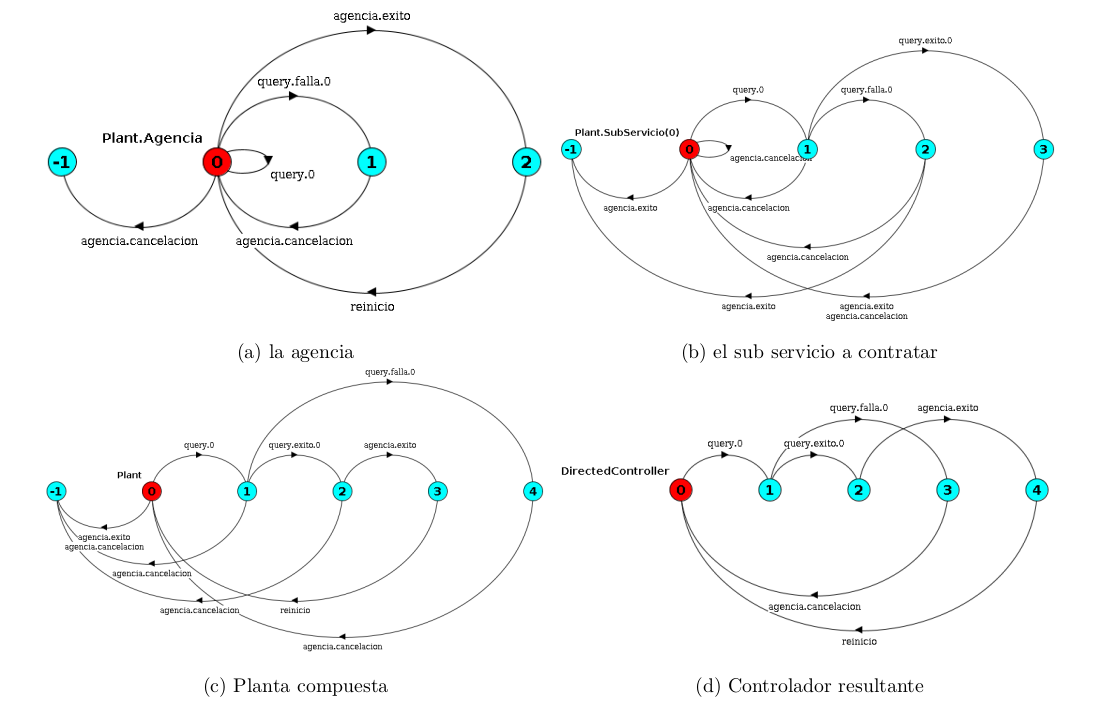
\includegraphics[width=1\textwidth]{capitulos/cap1/img/TAEjemploMTSA.png}
    \caption{Ejemplo del problema Travel Agency (TA) con un solo sub-servicio}
    \label{fig:ejemploTAProblema}
\end{figure}

En el ejemplo, la figura \ref{fig:ejemploTAProblema}a es la representación de la agencia que busca confirmar la compra, el estado 2 es nuestro estado marcado, objetivo que queremos alcanzar infinitas veces. En cambio, al detectar algún \textit{query.falla}, se mueve al estado 1, señalando que hubo un problema y solo permite cancelar la compra de todos los otros servicios consultados.

El componente del \textit{subservicio} (figura \ref{fig:ejemploTAProblema}b) también tiene el evento \textit{agencia.exito}, pero debe previamente haber recibido la consulta y confirmado su disponibilidad tomando el evento \textit{query.exito.0}. 

En caso de no ser posible la reserva, solo permite la cancelación de la compra, yendo del estado 2 al 0; si se
quisiera confirmar la compra (\textit{agencia.exito}) se llega al \textbf{estado -1}, reservado para los errores
que el controlador debe evitar.

Podemos observar la representación del sistema complejo en la sincronización que se ve reflejada en la figura \ref{fig:ejemploTAProblema}c, que muestra la planta que representa al sistema con los dos componentes previamente descriptos.

Finalmente, \ref{fig:ejemploTAProblema}d muestra un posible controlador para este problema. Destacamos que todos los eventos controlables que llevaban al estado -1 (el estado error), no son una posibilidad permitida por el controlador.

\begin{figure}[h!]
    \centering
    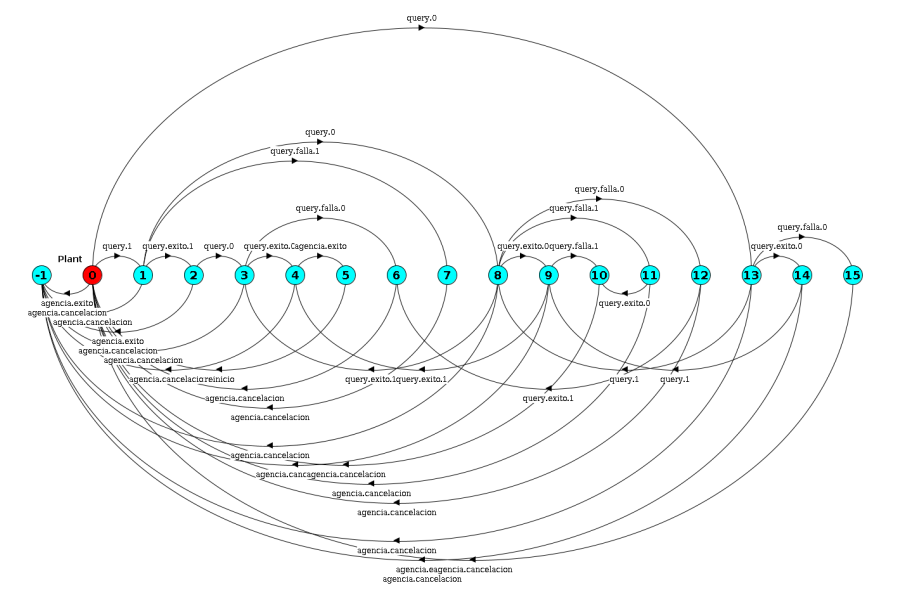
\includegraphics[width=.85\textwidth]{capitulos/cap1/img/EjemploTACompuestoMTSA.png}
    \caption{Planta compuesta para 2 sub-servicios}
    \label{fig:ejemploTAPlanta}
\end{figure}

\FloatBarrier

Si analizamos el tamaño que adquiere la planta compuesta expresada en la figura \ref{fig:ejemploTAPlanta} podemos notar que es un tipo de problema que escala rápidamente cuando se incrementan los autómatas que se van a componer. También podemos ver que el controlador posee un subconjunto de estados y transiciones de la planta compuesta total. 

Por esta razón reafirmamos el enfoque de exploración \textit{on-the-fly} para resolver el problema de síntesis evitando, en la medida de lo posible, la composición de todo el modelo. 

\vspace{5cm}



%% Capítulo 3
\chapter{Branching bisimilarity}

% =====================================================================
% ESTRUCTURA OBJETIVO DE ESTE CAPÍTULO (ver planificacion-tesis.md)
%   3.1 Definición formal.
%   3.2 Relación con otras equivalencias (weak, observational, WSOE)
%       -> clave para justificar la sustitución del Cap. 4.
%   3.3 Algoritmo O(m log n) de Groote et al. (2019):
%       ideas principales, estructuras (splitters, bloques), invariantes.
%
% Papers de referencia:
%   - Groote, Jansen, Keiren, Wijs (2019), arXiv:1909.10824  -> \cite{groote2019}
%     (copia local en Papers/jansen.pdf)
% =====================================================================

% TODO(intro): párrafo puente desde el Cap. 2. Recordar que en el flujo
% composicional se minimiza entre composiciones usando una noción de
% equivalencia (WSOE, definida en 2.4) y que el costo de esa minimización
% es el cuello de botella. Anunciar que branching bisimilarity es la
% equivalencia candidata a reemplazarla y que este capítulo la define,
% la ubica frente a las equivalencias clásicas y presenta el algoritmo
% eficiente que la calcula.

\section{Definición formal}

% TODO(3.1):
%  - Definir transiciones internas / no observables (acción tau) sobre el
%    LTS ya definido en el Cap. 2; introducir notación si hace falta
%    (reusar \step, \walk, \hop de commands.tex en lugar de inventar).
%  - Definición de branching bisimulation entre dos estados: condición de
%    matching que permite intercalar pasos tau preservando el estado
%    intermedio (la diferencia clave con weak bisimulation).
%  - Branching bisimilarity como la mayor branching bisimulation; mencionar
%    que es relación de equivalencia.
%  - (Opcional) variante divergence-sensitive si se usa en el contexto
%    composicional; aclarar cuál se adopta y por qué.
%  - Ejemplo mínimo: dos LTS branching-bisimilares y un par que NO lo es
%    pero sí es weak-bisimilar (motiva 3.2).

\section{Relación con otras equivalencias}

% TODO(3.2): este es el puente conceptual hacia el Cap. 4.
%  - Ubicar branching bisimilarity en la jerarquía: strong > branching >
%    weak / observational. Dar la intuición de por qué branching es más
%    fina que weak (preserva el potencial de los estados intermedios).
%  - Relación con observational equivalence.
%  - Relación con WSOE (la noción del paper composicional, definida en 2.4):
%    adelantar la afirmación que el Cap. 4 demuestra formalmente y dar la
%    intuición de por qué coinciden en el contexto de control.
%  - Cerrar motivando: si coinciden en lo que importa para síntesis, se
%    puede sustituir WSOE por branching bisimilarity y ganar el algoritmo
%    eficiente de 3.3.

\section{\texorpdfstring{Algoritmo $O(m \log n)$}{Algoritmo O(m log n)} de Groote et al.}

% TODO(3.3): basado en \cite{groote2019} (Papers/jansen.pdf).
%  - Idea general: partition refinement. Partir de una partición inicial
%    de los estados en bloques y refinarla hasta el punto fijo.
%  - Estructuras de datos clave: bloques, partición refinable, splitters,
%    y la maquinaria que da la cota O(m log n) (estrategia "process the
%    smaller half" / constellations-bloques del paper).
%  - Invariantes que mantiene el refinamiento (estabilidad de bloques
%    respecto de los splitters) y por qué garantizan correctitud.
%  - Complejidad: enunciar O(m log n) (m transiciones, n estados) y
%    contrastar con la complejidad de la minimización por WSOE vista en
%    2.4 -> ESTE es el argumento de escalabilidad de toda la tesis.
%  - El pseudocódigo extendido va al Apéndice; acá solo las ideas y
%    estructuras principales (usar el lstdefinelanguage 'pseudocode' de
%    tesis.tex si se incluye algún fragmento).
%  - Nota: la adaptación concreta de este algoritmo al contexto
%    composicional (eventos controlables/no-controlables, estados
%    marcados) y su implementación se tratan en el Cap. 5.


%% Capítulo 4
\chapter{Definición y análisis de las Fases de Exploración}
\section{Explicación general}
Durante el proceso de síntesis del controlador que realizamos mediante la exploración on-the-fly de la planta notamos que se atraviesan ciertas etapas (o fases) cuyos objetivos parciales no siempre coinciden, más allá de ser etapas que conducen a un objetivo en común (resolver el problema de control en general). La exploración atraviesa estas etapas de forma totalmente agnóstica a la heurística elegida porque están relacionadas directamente con la estructura del algoritmo de exploración dirigida.

% En el capítulo anterior concluímos que la heurística RA definida consigue buenos resultados para aproximar las mejores transiciones a explorar durante el algoritmo on-the-fly. Describimos el funcionamiento mediante el que consigue, para cada estado $e$ dentro de los estados explorados, estimar el número de pasos necesarios para alcanzar un estado marcado. De esa forma, la heurística RA posee la ventaja de representar las estructuras necesarias para su funcionamiento con una representación reducida del estado de espacios que deshecha mucha información pero conserva la suficiente para realizar la estimación mencionada.  Esta representación reducida de alguna manera nos permite abordar de forma eficiente el problema referido como \textit{explosión de estados}, en el que cae la solución Monolítica y genera complicaciones vistas en \cite{1}
% \\
% En ese sentido, entendemos que la importancia de esta heurística nos resulta particularmente útil para la etapa inicial del problema de síntesis de un \textit{Controlador}, que requiere la alcanzabilidad de un primer estado marcado.


\section{Definición de las fases de exploración}

Vamos a definir cuatro fases que creemos importantes considerar a la hora de elegir una heurística para el problema de control general. Los puntos claves que las definirán son: encontrar el primer estado marcado, cerrar un ciclo \textit{exitoso}, concluir que el ciclo encontrado previamente sea controlable y finalmente la propagación hasta el estado inicial de la condición de controlabilidad.

\subsection{Fase 1: encontrar un estado marcado}

Consideramos como parte de la \textit{Fase 1} de exploración a todas las transiciones y estados expandidos antes de realizar la primera transición cuyo destino sea un estado marcado. Tomamos esa definición porque hasta no encontrar un primer estado marcado en nuestra exploración, por definición tampoco podríamos definir estados \textit{ganadores} como \textbf{Goal} entre los explorados. En principio, nuestro enfoque realiza una exploración que parte desde un estado inicial y busca encontrar un ciclo que satisfaga la condición \textit{\textbf{canBeWinningLoop}}. Como vimos anteriormente, la condición exige que el ciclo que evaluamos contenga un estado marcado o que algún estado dentro del mismo pueda alcanzar en un paso a otro estado catalogado como \textbf{Goal}. En ese sentido definimos formalmente a la \textbf{Fase 1} de exploración como el lapso hasta que expandamos una transición hacia un estado marcado por primera vez.

\begin{figure}[h!]
    \centering
    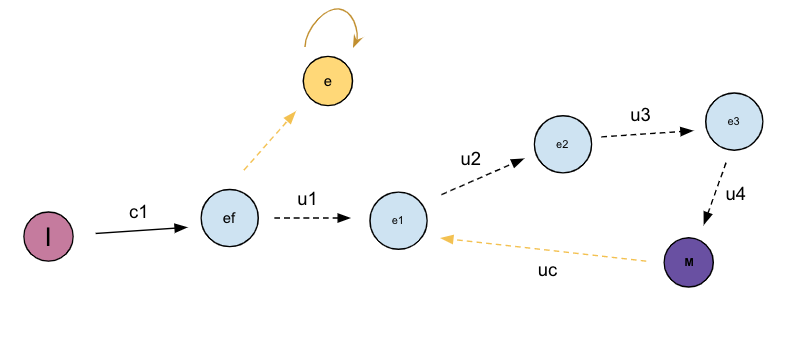
\includegraphics[width=.65\textwidth]{capitulos/cap4/img/fase1/ejemploFase1.png}
    \caption{Ejemplo de exploración que finaliza la Fase 1}
    \label{fig:fase1Ejemplo}
\end{figure}

En la figura \ref{fig:fase1Ejemplo} se puede ver como se requirieron explorar \textbf{5 estados} a través de \textbf{5 transiciones} llamadas \textit{c1, u1, u2, u3} y \textit{u4}.

% \FloatBarrier

\subsection{Fase 2: cerrando un ciclo \textit{exitoso}}

Luego de haber expandido una transición que llegue a un estado marcado y habiendo completado la \textbf{Fase 1} que fue descripta anteriormente, buscaremos que se cierre un ciclo sobre ese estado marcado que exploramos. Como podemos ver en el pseudocódigo del algoritmo principal, la función  requiere expandir una transición que cierre un ciclo dentro del total de estados explorados. Lo que buscamos será verificar formalmente la noción de cierre de ciclo. Para eso, si expandimos la transición $(e, e')$, en principio queremos chequear la siguiente condición: $\exists w \ \ldot e' \runw{w}{\structure'} e.$ \\ 
Es decir aseguramos la existencia de un camino $w$ mediante el cual alcancemos $e$ desde $e'$. En la línea siguiente vamos a conseguir, mediante la función auxiliar \textbf{getMaxLoop}, un conjunto con todos los estados que forman parte del ciclo cuya existencia aseguramos en el paso anterior. \\
Una vez que hayamos chequeado afirmativa esa condición, necesitamos hacer una segunda verificación acerca de ese ciclo en donde nos aseguramos parcialmente ciertas condiciones adicionales que en caso no cumplirse nos obligarían a descartarlo. \\
Esta segunda verificación se encuentra formalizada como función auxiliar en nuestro pseudocódigo con el nombre de \textbf{canBeWinningLoop}, función que toma un conjunto de estados que forman un ciclo y chequea la posibilidad de alguna de estas dos condiciones: que exista un estado marcado dentro de ese ciclo, o que exista algún estado dentro del ciclo evaluado que pueda alcanzar en un paso a un estado etiquetado como \textit{Goal} dentro de la exploración. En nuestro caso, como estamos ejecutando un punto del algoritmo DCS donde aún no hay estados \textit{Goals} dentro de la exploración, tendremos que verificar la primera condición. \\
En el caso de verificar exitosamente la condición expresada en la función \textbf{canBeWinningLoop} de nuestro pseudocódigo habremos encontrado un ciclo potencialmente exitoso y concluímos la \textbf{Fase 2} ejecutando, por primera vez en el algoritmo DCS, la función \textbf{findNewGoalsIn} para ese mismo ciclo.

\begin{figure}[h!]
    \centering
    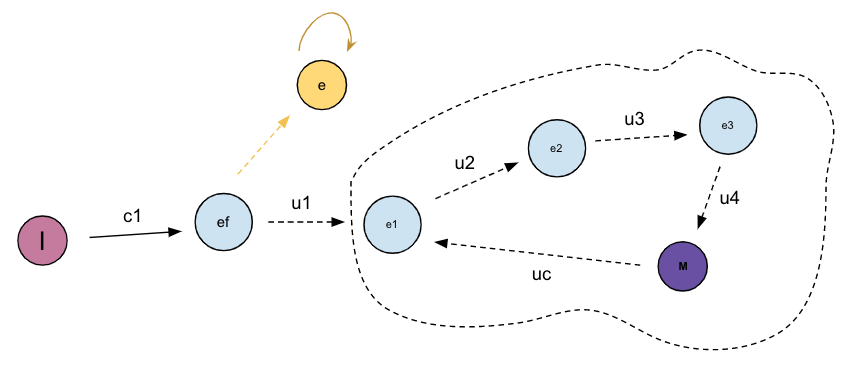
\includegraphics[width=.65\textwidth]{capitulos/cap4/img/fase2/ejemploFase2.png}
    \caption{Ejemplo de exploración que finaliza la Fase 2}
    \label{fig:fase2Ejemplo}
\end{figure}

En la figura \ref{fig:fase2Ejemplo} podemos ver que exploramos una transición adicional que no habíamos transitado en la figura \ref{fig:fase1Ejemplo}, la transición no controlable etiquetada como \textbf{uc}. Esta transición podemos ver que cierra un ciclo entre los estados \textit{e1, e2, e3 y M}, pero además es un ciclo \textit{exitoso} que garantiza la condición pedida por el método \textbf{canBeWinningLoop} ya que \textbf{M} es un estado marcado dentro del ciclo.

\subsection{Fase 3: garantizando controlabilidad del ciclo}

Esta fase comienza con la primera ejecución de la función \textbf{findNewGoalsIn} descripta en el pseudocódigo y usando como parámetro el ciclo que encontramos en la fase anterior. Esta función aplica un método de punto fijo que permite encontrar, en caso de que exista, un subciclo controlable a partir del ciclo original. Aunque los detalles y la formalización de la función están explicados en el pseudocódigo, es importante mencionar que para garantizar la \textit{controlabilidad} del ciclo se aplica iterativamente un proceso que quita algunos estados del conjunto que compone el ciclo original con cierto criterio. La idea será remover iterativamente estados que \textit{rompan} la controlabilidad del ciclo y buscar el conjunto de estados resultantes al momento en que, ante una nueva corrida, no se puedan eliminar más estados del conjunto. \\
El criterio mencionado para remover iterativamente estados del conjunto original se basa en cumplir alguna de las siguientes dos condiciones sobre cada estado $s \in C$, siendo $C$ el ciclo analizado:

\begin{enumerate}
    \item $\exists e \ldot forcedTo(s, e, \unexploredToBottom{\structure'}) \wedge e \notin (C \cup Goals)$
    \item  $\nexists s' \in C , \exists \l \ldot s' \step{\l}{\structure'} s$
\end{enumerate}
df
El punto 1 formaliza la primera razón para \textit{remover} elementos del ciclo analizado durante la ejecución de \textbf{findNewGoalsIn}. La fórmula expresa que no puede haber ningún estado dentro del ciclo que esté forzado a irse mediante una transición no controlable a un estado $e$ que no esté en el ciclo ni haya sido previamente marcado como \textit{Goal}. 

El punto 2 expresa la condición de ser un estado no alcanzable por ningún otro estado dentro del ciclo. En la primera iteración del método ningún estado cumplirá esta condición ya que el parámetro (un conjunto de estados que conforma un ciclo) conforma un grafo conexo. Una vez que empecemos a quitar elementos de este conjunto por cumplir la condición expresada en punto 1 aparecerán ciertos estados no alcanzables desde ningún otro estado del ciclo, es decir que cumplen la condición número 2.

\begin{figure}[h!]
    \centering
    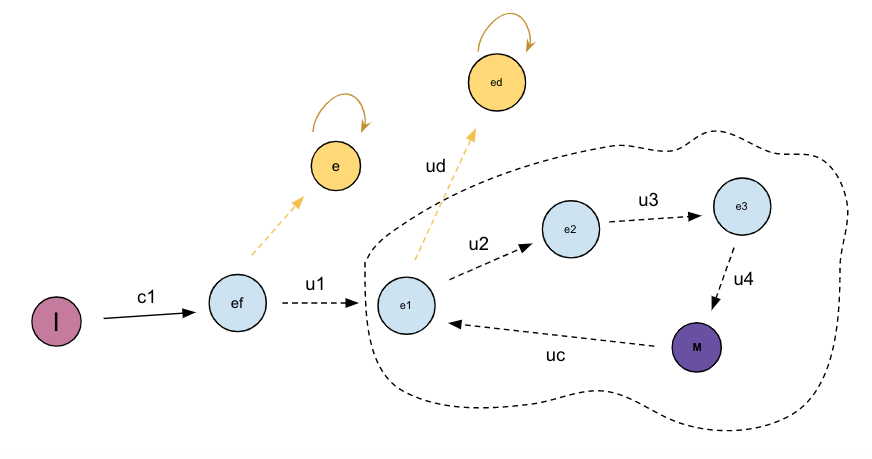
\includegraphics[width=0.65\textwidth]{capitulos/cap4/img/fase3/ejemploFTL1.png}
    \caption{Ejemplo de un ciclo (rodeado por línea de puntos)}
    \label{fig:ejemploFTL}
\end{figure}

\FloatBarrier
En la figura \ref{fig:ejemploFTL} podemos ver un ejemplo en donde la línea punteada encierra un ciclo que contiene un estado marcado y cuyos estados que lo componen serán parámetro de la función \textbf{findNewGoals}. Luego, al ejecutarse esta función y analizar los estados que componen el ciclo, encontrará que el estado \textit{e1} es un estado que cumple la primera de las condiciones que enumeramos anteriormente, ya que posee una transición no controlable \textbf{(ud)} hacia un estado $ed$ que no se encuentra dentro del ciclo ni está dentro del conjunto de estados marcados como \textit{Goal}. En ese sentido, el estado $e1$ será removido como parte de la primera iteración del método \textbf{findNewGoals}, dando lugar a una estructura reflejada en la figura \ref{fig:ejemploFTL2}. 

\begin{figure}[h!]
    \centering
    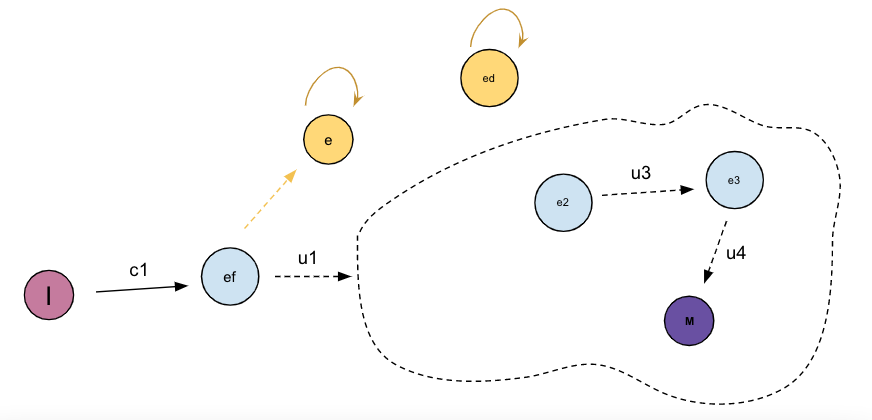
\includegraphics[width=0.65\textwidth]{capitulos/cap4/img/fase3/ejemploFTL2.png}
    \caption{Ejemplo del ciclo luego de remover en una iteración los estados del ciclo que cumplían la condición 1}
    \label{fig:ejemploFTL2}
\end{figure}

Lo que podemos ver en la figura \ref{fig:ejemploFTL2} es el conjunto resultado de la primera iteración del método \textbf{findNewGoals} luego de eliminar el estado que mencionamos anteriormente y que destacamos en la figura \ref{fig:ejemploFTL}. De esta manera destacamos al estado $e2$ que se puede ver como no cumple la condición número dos de las enumeradas previamente porque justamente se trata de un estado que, en esta iteración, ni siquiera recibe transiciones entrantes. Por lo tanto podemos determinar que no será alcanzable desde ningún estado, lo que implica que tampoco será alcanzable por un estado del ciclo.
\\
Para el ejemplo citado en las figuras, el algoritmo de punto fijo sobre el conjunto que representa al ciclo resultará con un conjunto vacío ya que todos los estados serán removidos por alguna de las condiciones comentadas previamente. Podemos ver en el pseudocódigo correspondiente a \textbf{findNewGoals} que en ese caso devolvería un conjunto vacío que no genera ningún cambio a nivel general de la ejecución del algoritmo DCS. Justamente lo que buscamos en esta fase es lograr un subciclo controlable como resultado de nuestro método, en donde exista una iteración que ya no modifique el conjunto y a la vez haya elementos que compongan el subciclo buscado. 
\\
% Acá definimos los conjuntos que se particionan en el FNG
En este sentido conviene analizar en mayor profundidad las razones por las cuales el resultado de la ejecución del método \textbf{findNewGoals} no resulta exitosa (es decir devuelve un conjunto vacío) y eso lo haremos, en principio, caracterizando algunos tipos de estados que se desprenden de la lógica del método iterativo.
\\
En principio analizaremos los estados del ciclo que es parámetro del método \textbf{findNewGoals} que cumplen con la condición de estar \textit{forzados a irse} y que formalizamos previamente. La idea de este análisis será ver que características nos permiten agrupar a esos estados. 
\\
Por un lado, nos interesa analizar los estados forzados a irse \textbf{en la primera iteración} del método \textbf{findNewGoals}. Es importante chequear esta condición en la primera iteración ya que después el método funciona quitando elementos del conjunto, por lo cual en posteriores iteraciones se pueden encontrar transiciones no exploradas por haber removido previamente al destinatario de alguna de esas transiciones. Estos estados que el método quita en la primera iteración del conjunto son los que desencadenan el resultado negativo sobre el chequeo de controlabilidad del ciclo. Podemos afirmar que, en caso de \textit{resolver} las transiciones de esos estados que \textit{lo sacan} del ciclo, hubieramos encontrado un subciclo controlable como resultado del método \textbf{findNewGoals}.

\begin{figure}[h!]
    \centering
    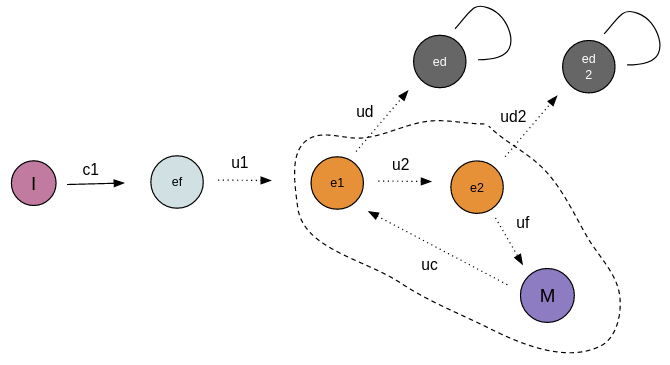
\includegraphics[width=0.65\textwidth]{capitulos/cap4/img/fase3/ejemploFTL3.png}
    \caption{Ejemplo del ciclo evaluado en la primera iteración del método FindNewGoalsIn}
    \label{fig:ejemploFTL3}
\end{figure}

En la figura \ref{fig:ejemploFTL3} y dentro del círculo punteado representamos el estado del ciclo que será evaluado en la primera iteración del método \textbf{findNewGoalsIn}. Destacamos dentro del ciclo a los estados \textbf{e1} y \textbf{e2} ya que ambos poseen transiciones no controlables \textit{(ud y ud2 respectivamente)} que conducen a estados que están por fuera del ciclo y que no están catalogados como Goal, de hecho son estados Deadlock. Queremos analizar puntualmente a los estados que cumplen esta condición ya que son claves para la resolución de esta fase de exploración. La importancia de estos estados está justificada en el hecho de suponer -para el ejemplo de la figura \ref{fig:ejemploFTL3}- que si las transiciones \textbf{ud} y \textbf{ud2} condujeran a caminos controlables que \textit{vuelvan} al ciclo entonces resolveríamos el problema de control planteado en \textbf{findNewGoalsIn}. La Fase 3 finaliza cuando el problema de controlabilidad del ciclo sea resuelto y encontremos un subciclo controlable, el cual nos servirá de parámetro para empezar la Fase 4.

\subsection{Fase 4: propagación de estados Goal}

Concluímos la fase anterior devolviendo un subciclo controlable que contiene un estado marcado. Este proceso es condición necesaria para resolver nuestro problema en general ya que nos permite lograr no solo alcanzabilidad a un estado marcado, sino también una manera de llegar de forma controlable a el. Por como fue definido el problema de control previamente, partimos la exploración desde un estado inicial desde el cual tenemos que poder alcanzar, también controlablemente, el subciclo mencionado.
\\
La Fase 4 inicia con la primera ejecución del método \textbf{propagateGoal}, cuyo parámetro será el ciclo controlable que encontramos en la fase anterior. Este método buscará garantizar que podamos llegar controlablemente desde el estado inicial hacia alguno de los estados del ciclo.
\\
Por lo tanto, primero buscaremos encontrar todos los estados \textit{ancestros} explorados que no hayan sido etiquetados como \textit{Goal} o \textit{Error} de los elementos del ciclo mediante el método \textbf{ancestorsNone}. Los \textit{ancestros} conseguidos mediante esta función se formalizan con el siguiente conjunto:

\vspace{.5cm}

\begin{center}
$\{ \, e \in \Review{\structure'} \mid \exists e' \in ciclo \ldot \exists w \ldot \trimlst{e \runw{w}{\Review{\structure'}} e'} \wedge$
          $ \nexists s \in \Review{w(e)} \ldot \Review{s \neq e' \wedge } s \in \Goals \cup \Errors \}$
\end{center}

\vspace{.5cm}

Sobre este nuevo conjunto de estados \textit{ancestros} del ciclo controlable y etiquetados como \textbf{None}, realizaremos un proceso iterativo similar al de la fase anterior en donde vamos a remover estados que cumplan con algunas de las siguientes condiciones:

\begin{itemize}
    \item Quitaremos estados que en el proceso de propagación encontremos que estén \textit{forzados a irse}. Esto quiere decir que son estados que tienen transiciones no controlables hacia elementos que no están en el ciclo ni hayan sido etiquetados como Goal previamente. 
    Estos estados se pueden describir formalmente para todos los estados $s \in ancestorsNone(estadosCiclo)$ de la siguiente manera:
    \begin{center}
        \textbf{forcedTo}($s, S_{\unexploredToBottom{\structure'}}\setminus (C \cup \Goals),\unexploredToBottom{\structure'}$)
    \end{center}
    
    \item Por otro lado también vamos a remover iterativamente los estados que no puedan alcanzar un estado \textbf{Goal} y cuya condición se describe formalmente en la siguiente línea cuya definición más extensa encontraremos en el pseudocódigo:
    \begin{center}
        $\neg$\textbf{canReachGoalIn}($s, C,\unexploredToBottom{\structure'}$)
    \end{center}

\end{itemize}

\vspace{.5cm}

\begin{figure}[h!]
    \centering
    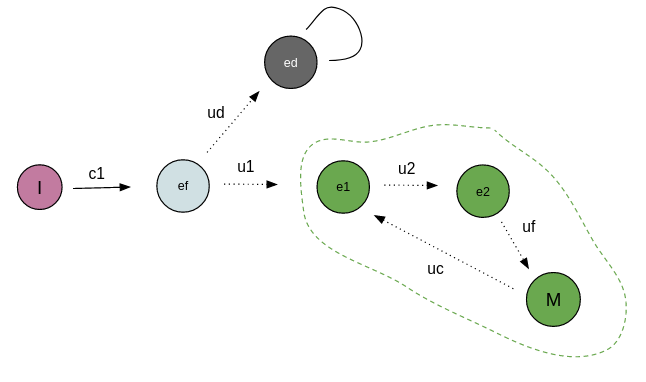
\includegraphics[width=0.7\textwidth]{capitulos/cap4/img/fase4/ejemploPropFallido.png}
    \caption{Ejemplo de proceso de PropagateGoal fallido}
    \label{fig:propGoalFallido}
\end{figure}

\FloatBarrier

En la figura \ref{fig:propGoalFallido} podemos ver un caso en donde ejecutamos el método \textbf{propagateGoal} habiendo completado la Fase 3 por encontrar un subciclo controlable con un estado marcado (marcado con línea de puntos resaltada en verde). Sin embargo, el proceso de propagación iniciado desde todos los estados del ciclo falla al llegar al estado \textit{ef}, el cual tiene una transición no controlable \textbf{ef} saliente hacia un estado \textbf{marcado como deadlock}. 
\\
En ese sentido buscamos caracterizar los estados que nos llevan a \textit{perder} en el proceso de la \textbf{Fase 4} por no lograr una propagación controlable hacia el estado inicial. Este análisis nos puede dar algunos indicios de cara a la elaboración de una estrategia que minimice las ejecuciones de \textbf{propagateGoal}. En principio no encontramos características en las heurísticas con las que venimos trabajando \textit{(Random, BFS, RA)} que utilicen esta información de cara a elegir transiciones para la exploración. Este aspecto nos motivará de cara a la siguiente sección, en la cual buscaremos variantes de las heurísticas existentes que permitan utilizar nueva información.

\begin{figure}[h!]
    \centering
    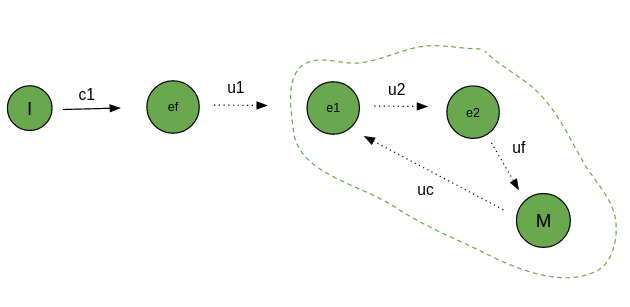
\includegraphics[width=0.7\textwidth]{capitulos/cap4/img/fase4/ejemploPropExitoso.png}
    \caption{Ejemplo de proceso de PropagateGoal exitoso}
    \label{fig:propGoalExitoso}
\end{figure}

\FloatBarrier

En la figura \ref{fig:propGoalExitoso} podemos ver en cambio un caso en donde concluye exitosamente la Fase 4. El ciclo controlable es idéntico al planteado en la figura \ref{fig:propGoalFallido}, al igual que el principio de la propagación que busca hacer esta fase. La diferencia está en haber sacado la transición no controlable etiquetada como \textit{ud} que incluíamos en la figura \ref{fig:propGoalFallido} y que convertía en no controlable el camino que recorríamos en la propagación desde el ciclo hasta el inicial.

\newpage
\section{Peso de las etapas en la exploración}
\subsection{Descripción de los casos de estudio}
En la siguiente \textit{subsección} mostramos los resultados de una experimentación que nos permitirán medir el peso relativo que tiene cada una de las etapas descriptas anteriormente en el proceso de exploración general. Decidimos usar el mismo conjunto de problemas que el utilizado para examinar la performance del algoritmo original de síntesis en \cite{DuranZanollo}. A continuación describimos brevemente todos los casos de estudios, los cuales fueron escritos con la posibilidad de ser escalados en el número de componentes y estados:

\begin{itemize}
    \item \textbf{Transfer Line:} Automatización de una fábrica, un dominio de mucho interés en el área de supervisory control. \textbf{TL} consiste de \textit{n máquinas} conectadas por n buffers cada uno con capacidad de \textit{k unidades}, termina en una máquina adicional llamada Test Unit.
    
    \item \textbf{Dinning Philosophers:} Problema clásico de concurrencia. En \textbf{DP} hay \textit{n filósofos} sentados en una mesa redonda, cada uno comparte un tenedor con sus vecinos aledaños. El objetivo del sistema es controlar el acceso a los tenedores de manera que los filósofos puedan alternar entre comer y pensar; evitando deadlock y starvation. Adicionalmente, cada filósofo, luego de tomar un tenedor, debe cumplir con \textit{k pasos de etiqueta} antes de comer.
    
    \item \textbf{Cat and Mouse:} Juego de dos jugadores donde cada uno toma turnos para moverse a una casilla adyacente dentro de un mapa de la forma de un corredor dividido en 2k + 1 áreas. En \textbf{CM} \textit{n gatos y la misma cantidad de ratones} son colocados en extremos opuestos del corredor. El objetivo es mover a los ratones de manera que no terminen en el mismo lugar que un gato. Los movimientos de los gatos no son controlables. En el centro del corredor hay un agujero que lleva a los ratones a un área segura.
    
    \item \textbf{Bidding Workflow:} Modela el proceso de evaluación de proyectos de una empresa. El proyecto debe ser aprobado por \textit{n equipos}. El objetivo es sintetizar un flujo de trabajo que intente llegar a un consenso, es decir, aprobar/rechazar el proyecto cuando todos los equipos lo aceptan/rechazan. La propuesta puede ser reasignada para reevaluación por un equipo hasta \textit{k veces}, no se puede reasignar si el equipo ya lo habı́a aceptado. Cuando un equipo \textit{lo rechaza k veces} el proyecto puede ser rechazado sin consenso. Es un caso de estudio tı́pico del dominio de Business Process Management.
    
    \item \textbf{Air-Traffic Management:} Representa la torre de control de un aeropuerto, que recibe \textit{n peticiones} de aterrizaje simultáneas. La torre necesita avisar si tiene permiso para aterrizar o, en caso contrario, en cuál de los \textit{k espacios aéreos} debe realizar maniobras de espera. El objetivo es que todos los aviones puedan aterrizar de manera segura. El problema solo tiene solución si la cantidad de aviones es menor a la de espacios aéreos (n $<$ k).
    
    \item \textbf{Travel Agency:} Modela una página on-line de ventas de paquetes de viajes. El sistema depende de \textit{n servicios} de terceros para realizar las reservas (ej. alquiler de auto, compra de pasajes, etc). Los protocolos para utilizar los servicios pueden variar de manera no controlable; una variante es la selección de hasta \textit{k atributos}(ej. destino del vuelo, clase y fechas). El objetivo del sistema es orquestar los servicios de manera de obtener un paquete de vacaciones completo de ser posible, evitando pagar por paquetes incompletos.
\end{itemize}

Por otro lado, para medir la performance del benchmark descripto utilizamos el registro de tiempo total, transiciones expandidas y estados expandidos al finalizar la exploración. Todos estos resultados los estaremos midiendo, finalmente, para dos heurísticas que nos permitan realizar una comparación exploratoria sobre su impacto en las fases. Estas dos heurísticas que guían la exploración serán Breadth First Search (BFS) y RA \cite{Ciolek}. Descartamos la utilización en este caso de una heurística Random debido al elevado numero de ejecuciones requeridas para tener resultados con estadística ya que las ejecuciones no son deterministas, y debido a que BFS y RA superan en \textit{performance} a Random (podemos verlo en \cite{DuranZanollo}, por lo cual esas heurísticas nos alcanzan como base.

\subsection{Resultados}

Sabemos que cada heurística tiene distintos pesos relativos sobre cada una de las fases comentadas como se puede ver en las tablas que figuran en el anexo de este trabajo. Para poder comparar el peso relativo de cada una contrastaremos los dos tipos de heurísticas más exitosas según el trabajo visto en \cite{Ciolek} que son RA y BFS.

En la tabla \ref{tab:estadosravsbfsporc} podemos ver, para cada caso de estudio, el porcentaje de instancias en las que la heurística RA explora menos estados que la heurística BFS. Consideramos únicamente las instancias que son resueltas por ambas heurísticas garantizando soluciones controlables al problema de síntesis.

\begin{table}[h!]
\begin{center}
\begin{tabular}{| c | c | c | c | c | c | c | }
\hline
\multicolumn{7}{ |c| }{Performance de estados explorados por fase RA vs BFS} \\ \hline
Fase / Caso & TA & AT & BW & CM & DP & TL \\ \hline
Fase 1 & 33\% & 30\% & 80\% & 100\% & 100\% & 100\%  \\
Fase 2 & 33\% & 25\% & 84\% & 100\% & 100\% & 100\%  \\
Fase 3 & 100\% & 85\% & 84\% & 100\% & 100\% & 100\% \\
Fase 4 & 100\% & 25\% & 100\% & 65\% & 100\% & 100\% \\
Total & 100\% & 85\% & 84\% & 100\% & 100\% & 100\% \\ \hline
\end{tabular}
\caption{Porcentaje de instancias que RA resuelve con menor cantidad de estados explorados que BFS por fase}
\label{tab:estadosravsbfsporc}
\end{center}
\end{table}

Los resultados que podemos ver en la tabla \ref{tab:estadosravsbfsporc} muestran que, considerando el total de estados expandidos, la heurística RA \textit{gana} sobre BFS en mas de un 84\% de las instancias analizadas para cada tipo de caso de estudio. Sin embargo, analizando por fases hay algunos casos donde RA pierde frente a BFS como podemos ver en Fase 1 y Fase 2 de TA y AT, y Fase 4 de AT.

Sin embargo, la tabla \ref{tab:estadosravsbfsporc} no nos brinda información cualitativa sobre en qué medida la heurística \textbf{RA} mejora en cantidad de estados explorados a la resolución que propone \textbf{BFS}. Para eso, proponemos analizar los datos utilizando un nuevo indicador. Definimos para una fase $f  \in \{1,2,3,4\}$ fija y dos heurísticas RA y BFS, el indicador \textbf{$I_f$} de la siguiente manera:

\vspace{1.2cm}

\[ I_f = 
\frac{\sum_{i \ \in \ Inst.} CantEstados_{RA}^{f}(i)}{
\sum_{i \ \in \ Inst.} CantEstados_{RA}^{f}(i) + 
\sum_{i \ \in \ Inst.} CantEstados_{BFS}^{f}(i)}
\]

\vspace{1.2cm}

Si consideramos que $CantEstados_{RA}^{f}(i)$ y $CantEstados_{BFS}^{f}(i)$ son funciones auxiliares que nos devuelven la cantidad de estados explorados en cada fase \textit{f} y para una instancia \textit{i} en ambas heurísticas. De esta forma, sumando y luego comparando el desempeño en el total de las instancias nos otorga una métrica con la que medimos cualitativamente \textit{cuanto mejor desempeño} tiene la heurística RA sobre BFS por fase. 

% Si expresamos este valor porcentualmente en términos del esfuerzo conjunto de ambas heurísticas para resolver una fase, una coordenada de esta tabla será el porcentaje de estados totales que usa \textbf{RA} obtuvo como desempeño en cuanto a \textbf{BFS}. 

A continuación otorgamos una descripción más precisa acerca del significado que tienen los posibles valores de este indicador y que los podemos interpretar de la siguiente manera:

{\centering
\vspace{0.7cm}

I_f \cong \left\{ \begin{array}{lcc}
            \\ 0 &  si  & \textbf{RA} \ $no explora estados en esa fase$ \\
            \\ 0 \  \textless \ I_f \ \textless \ 0.5 &  si  & \textbf{RA} \ $explora \textbf{menos} estados que \textbf{BFS} en esa fase$ \\
            \\ 0.5 &  si  & \textbf{RA} \ $explora \textbf{igual} cantidad de estados que BFS en la fase$ \\
            \\ 0.5 \  \textless \ I_f \ \textless \ 1 &  si  & \textbf{RA} \ $explora \textbf{más} estados que \textbf{BFS} en esa fase$ \\
            \\ 1 &  si  & \textbf{BFS} \ $no explora estados en esa fase$ 
            
             \end{array}
   \right.

\centering}

\vspace{0.7cm}

Luego de haber definido este nuevo indicador, veremos en la tabla \ref{tab:estadosravsbfscomparacion} los resultados de esta métrica expresada para todos los casos y diferenciada por fase. Particularmente en los casos donde \textbf{ninguna de las dos heurísticas} utilice ningún estado para resolver una fase pondremos un guión como referencia en la tabla.

\vspace{0.3cm}

% Acá la idea es poner la sumatoria de transiciones de cada fase para todas las instancias usando heurística RA sobre usar BFS.
\begin{table}[h!]
\begin{center}
\begin{tabular}{| c | c | c | c | c | c | c | }
\hline
\multicolumn{7}{ |c| }{Performance de estados explorados por fase RA vs BFS} \\ \hline
Fase / Caso & TA & AT & BW & CM & DP & TL \\ \hline
Fase 1 & 0,63 & 0,32 & 0,27 & 0,08 & 0,01 & 0,01  \\
Fase 2 & 0 & 0,007 & 0 & 0,01 & 0 & 0  \\
Fase 3 & 0,27 & 0,69 & 0,51 & 0,09 & 0,004 & 0,001 \\
Fase 4 & - & - & - & 1 & 0,06 & -  \\
Total & 0,28 & 0,42 & 0,42 & 0,2 & 0,007 & 0,006 \\ \hline
\end{tabular}
\caption{Indicador $I_f$ definido para cada caso del Benchmark y Fase definida}
\label{tab:estadosravsbfscomparacion}
\end{center}
\end{table}

\vspace{0.3cm}

En principio conviene remarcar de la tabla \ref{tab:estadosravsbfscomparacion} como \textit{RA} supera en \textit{performance} a \textit{BFS} en todos los casos obteniendo valores cercanos a cero para la etapa 2 y reduciendo los tiempos del resto de las etapas, salvando excepciones como la fase 1 de \textbf{TA} y las fases 3 de \textbf{BW} y \textbf{AT}, donde tenemos valores superiores al 0,5. Particularmente los casos \textbf{DP} y \textbf{TL} obtienen, usando \textit{RA}, resultados significativamente mejores en cada una de sus fases.

Si bien observamos que en la \textbf{fase 1} para el caso \textbf{TA} \textit{BFS} logra una mejor performance y en los casos \textbf{AT} y \textbf{BW} la ventaja de \textit{RA} no es tan significativa, nos gustaría poder ver en cual etapa hay un espacio de mejora. Si bien la tabla \ref{tab:estadosravsbfscomparacion} nos muestra la comparación de performance entre las dos heurísticas, no nos indica el costo de la fase en el total del algoritmo. Para eso analizaremos, para cada caso de estudio, el porcentaje de estados explorados por fase para la heurística RA. De esta forma tendremos una intuición acerca del peso relativo que tiene la ejecución de cada fase con determinada heurística.

% Tabla que contiene el porcentaje de cada fase para cada heurística
\begin{table}[h!]
\begin{center}
\begin{tabular}{| c | c | c | c | c | c | c | }
\hline
\multicolumn{7}{ |c| }{Porcentaje de cada fase medido mediante la acumulación de estados explorados para RA} \\ \hline
Fase / Caso & TA & AT & BW & CM & DP & TL \\ \hline
Fase 1 & 5\% & \textbf{56,3\%} & 17,5\% & 2\% & \textbf{84\%} & \textbf{93\%}  \\
Fase 2 & 0\% & 0,4\% & 0\% & 0,3\% & 0\% & 0\%  \\
Fase 3 & \textbf{95\%} & 43,3\% & \textbf{82,5\%} & 34\% & 14\% & 7\% \\
Fase 4 & 0\% & 0\% & 0\% & \textbf{63,7\%} & 2\% & 0\%  \\
Total & 100\% & 100\% & 100\% & 100\% & 100\% & 100\% \\ \hline
\end{tabular}
\caption{Porcentaje de cada fase medido en estados explorados para la heurística RA}
\label{tab:pesodefasesra}
\end{center}
\end{table}


% En \textbf{DP}, \textbf{TL} y \textbf{CM} se obtiene una gran ventaja en fase 1 y 2 para las cuales podemos ver en \cite{Ciolek} un análisis más detallado sobre como en estos casos RA hace una notoria diferencia en la \textit{performance} total. Particularmente vemos en este análisis preliminar de las fases de exploración que la heurística RA explota la ventaja de calcular la estimación de distancia hacia un estado marcado, lo que permitiría acelerar la etapa 1 con respecto a otras heurísticas. 

% Sin embargo, tanto para estos casos como para los otros tres cuya performance de la heurística \textbf{RA} es levemente inferior, podemos ver que la fase 3 es la que resulta más costosa. Si bien observamos que en la \textbf{fase 1} para el caso \textbf{TA} BFS logra una mejor performance y en los casos \textbf{AT} y \textbf{BW} la ventaja de \textbf{RA} no es tan significativa, podemos ver que hay un gran espacio de mejora en la \textbf{fase 3}. 

\FloatBarrier

En la tabla \ref{tab:pesodefasesra} encontramos, para cada caso de estudio, el porcentaje de estados explorados por fase usando la heurística RA. En la sección de \textbf{apéndice} encontraremos los gráficos en los que se mide el peso de cada etapa tanto para RA como podemos ver en la tabla, como para la heurística BFS.

La tabla  \ref{tab:pesodefasesra} nos proporciona una visión acerca de las fases más \textit{costosas} para resolver el problema de síntesis usando RA. Sin embargo, aunque este aspecto es valioso, es información que deberíamos complementar con la información anterior para buscar un nuevo indicador que nos de una idea de ventanas de mejora dentro de la experimentación realizada. Para eso planteamos una multiplicación de los valores de ambas tablas, con la idea de obtener un valor que combine ambos aspectos.

En este caso, un número alto implica que determinada combinación de fase y caso de estudio obtienen poca ventaja comparativa compitiendo contra BFS (el valor de la tabla \ref{tab:estadosravsbfscomparacion} y además eran originalmente difíciles de resolver para RA porque ocupaban gran porcentaje de los estados explorados en total (el valor en la tabla \ref{tab:pesodefasesra}).

% Tabla que contiene la multiplicación de tabla 4.2 y 4.3
\begin{table}[h!]
\begin{center}
\begin{tabular}{| c | c | c | c | c | c | c | }
\hline
\multicolumn{7}{ |c| }{Indicador de costo de las fases} \\ \hline
Fase / Caso & TA & AT & BW & CM & DP & TL \\ \hline
Fase 1 & 3,15 & 18,01 & 4,72 & 0,16 & 0,84 & 0,93  \\
Fase 2 & 0 & 0,003 & 0 & 0,003 & 0 & 0  \\
Fase 3 & \textbf{25,65} & \textbf{29,87} & \textbf{42,07} & 3,06 & 0,056 & 0,007 \\
Fase 4 & 0 & 0 & 0 & \textbf{63,70} & 0,12 & 0  \\ \hline
\end{tabular}
\caption{Multiplicación entre los valores de la tabla \ref{tab:estadosravsbfscomparacion} y la tabla \ref{tab:pesodefasesra}}
\label{tab:pesoponderado}
\end{center}
\end{table}

En la tabla \ref{tab:pesoponderado} se muestra explícitamente que la ventana de mejora para los problemas que le resultan \textit{más difíciles} (TA, AT, CM y BW) a la heurística \textbf{RA} se encuentra mayoritariamente en \textbf{fase 3} para TA, AT y BW y en \textbf{fase 4} para CM. Justamente los valores grandes en la tabla corresponden a que son problemas en donde la fase 3 era originalmente pesada de resolver para RA pero además tiene poca mejora sobre BFS (lo que corresponde a un valor de porcentaje alto en la tabla \ref{tab:estadosravsbfscomparacion}). 


Por lo tanto, podemos ver luego de estos análisis que existe una gran ventana de mejora a la heurística \textbf{RA} en su desempeño de la tercera etapa para la mayoría de los casos, sobresaliendo \textbf{TA}, \textbf{AT}, \textbf{BW} y \textbf{CM} en distinta escala.

Por último mencionamos el caso de \textbf{CM} donde podemos ver particularmente el problema de fase 4 expresado en períodos donde ejecuta repetidas veces el método \textbf{propagateGoal} sin éxito. Comparando este aspecto con los resultados obtenidos usando las heurísticas vemos que, aún logrando métricas totales parecidas, en RA se traslada el peso de la etapa 3 a la etapa 4. Esto indica que, en algunos casos particulares del problema CM, la heurística RA aporta a resolver rápido la fase 3 pero le cuesta terminar de propagar los estados Goal hasta que incluyan al inicial.

% Para empezar analizaremos el comportamiento de las fases de exploración para los casos TL y DP en donde podemos ver, para la heurística Random, como obtenemos una Fase 3 mayoritaria. Parte de esta experimentación está detallada en las figuras \ref{fig:dp_estados_random} y \ref{fig:tl_estados_random} Además de obtener las peores métricas comparando en general, este detalle indica la obvia falencia de esta heurística particularmente para cerrar ciclos controlables y exitosos en estos casos. 

% Además notamos que tanto las heurísticas BFS como RA presentan una predominancia en la Fase 1 que se puede ver expresado en las figuras \ref{fig:dp_estados_bfs} y \ref{fig:dp_estados_ra}, lo que indica que proporcionalmente estas heurísticas resuelven más rápido la controlabilidad de un ciclo ganador que el hallazgo del primer estado marcado de la exploración. En BFS se puede justificar esta demora en que la búsqueda a lo ancho puede abrir varias ramas de exploración sin mantenerse en la que nos acerque a encontrar un estado marcado. Por otro lado podemos ver en \cite{Ciolek} un análisis más detallado sobre como en estos casos RA hace una notoria diferencia en la \textit{performance} total. Particularmente vemos en este análisis preliminar de las fases de exploración que la heurística RA explota la ventaja de calcular la estimación de distancia hacia un estado marcado, lo que permitiría acelerar la etapa 1 con respecto a otras heurísticas. Sin embargo, en términos relativos vemos como resultan particularmente exitosos los casos de RA cuyas fases que requieran controlabilidad (fase 3 y fase 4) sean menores. 

% En cuanto al comportamiento de otros casos del \textit{benchmark} como BW, TA y CM se puede ver como para las tres heurísticas hay predominancia de etapa 3 en las métricas medidas como puede verse en las figuras \ref{fig:bw_estados_bfs}, \ref{fig:bw_estados_ra}, \ref{fig:bw_estados_bfs}, \ref{fig:cm_estados_bfs} y \ref{fig:bw_estados_bfs} \ref{fig:cm_estados_ra} .  Esto indica que la estructura de los problemas lleva a una deficiencia para garantizar controlabilidad del ciclo durante la exploración.

% Se puede observar que más allá del análisis de fases, estos casos son donde la heurística RA no logra una mejora significativa como en los mencionados anteriormente (TL y DP). Este resultado indica que la heurística RA no hace un aporte significativo en cuanto a resolver rápidamente el problema de las fases 3 y 4. 

% En el caso de CM podemos ver particularmente el problema de fase 4 expresado en períodos donde ejecuta repetidas veces el método \textbf{propagateGoal} sin éxito. Comparando este aspecto con los resultados obtenidos usando las heurísticas vemos que, aún logrando métricas totales parecidas, en RA se traslada el peso de la etapa 3 a la etapa 4. Esto indica que, en algunos casos particulares del problema CM, la heurística RA aporta a resolver rápido la fase 3 pero le cuesta terminar de propagar los estados Goal hasta que incluyan al inicial.


\subsection{Conclusiones}

En el análisis de resultados repasamos como el aporte de la \textbf{heurística RA} mejora la métrica del total de estados explorados para todos los casos. Sin embargo, si analizamos detalladamente, en los casos donde la mejora es menor comparativamente se puede ver que hay espacio de mejora en la fase 3 que, según el análisis que concluye en la tabla \ref{tab:pesoponderado}, es la que mayor cantidad de estados ocupa en resolver el problema en general. 

Por lo tanto sostenemos la hipótesis de la posibilidad de mejora para la tercera etapa de exploración por lo comentado anteriormente y considerando que, más allá de la estructura del problema, la heurística \textbf{RA} no utiliza información específica que lleve a resolver esa fase. 

A continuación haremos un análisis más detallado del comportamiento de la tercera etapa utilizando \textbf{RA} para encontrar elementos que nos permitan mejorar las métricas de exploración para esa fase.

%% Capítulo 5
\chapter{Implementación del algoritmo}

% Capítulo descriptivo: dónde encaja el algoritmo en el flujo composicional,
% cómo se construyó, qué decisiones de diseño se tomaron por sobre lo que
% deja abierto el paper, qué adaptaciones requirió el contexto de síntesis
% de controladores, y cómo se validó la correctitud.


\section{Introduccion}
% Una frase sobre qué es MTSA y por qué es la plataforma natural donde
% implementar el reemplazo de WSOE por branching bisimilarity.
La herramienta MTSA \cite{mtsa} es el framework de desarrollo realizado en Java para varias iniciativas de LaFHIS en el contexto de la investigacion sobre LTSs. Es por eso que tanto el algoritmo composicional presentado por Uchitel y Gagliardi \#AGREGAR CITA\# como la version de WSOE utilizada para la composicionalidad fueron implementados en esta herramienta. Era entonces natural realizar el desarrollo del algoritmo de Branching Equivalence sobre el mismo framework, ante la promesa de que esto reduciria la complejidad. A su vez, nos permitira comparar de forma mas veridica ambos algoritmos, realizando pruebas de Benchmarks tanto para tiempos de ejecucion como para el uso de memoria.

En primer lugar, se realizo la implementación del algoritmo de Branching Equivalence en el archivo BranchingEquivalence.java, creado en mtstools/DCS/Compositional/ ya que bajo este modulo estan las herramientas utilizadas por el algoritmo composicional.


A su vez, en CompositionalApproach.java se reemplazó la llamada original al algoritmo de WSOE por la llamada a la nueva funcion que utiliza el algoritmo de Groote y Jansen, reemplazando tambien los preprocesamientos necesarios para los algoritmos que se hacen en algunos casos fuera de las funciones principales.

La llamada al algoritmo de Branching Equivalence queda entonces de esta forma
\begin{lstlisting}[language=Java, numbers=none]                                
  Pair<List<Set<Long>>, List<Set<Triple<Long, String, Long>>>> branchingPartition
                    = BranchingEquivalence.getPartitions(localControllerMTS, localAlphabet, totalTranslator, goal.getFluents());

  MTS<Long, String> minimizationResult = BranchingEquivalence.buildMinimisedMTSFromPartition(localControllerMTS, tauLabels, translatorControllable, branchingPartition);
\end{lstlisting}                                                               

donde en la funcion getPartitions(...) se implementa el algoritmo de Groote y Jansen y se devuelve la partición final de estados y transiciones, y en buildMinimisedMTSFromPartition(...) se construye el MTS minimizado a partir de la partición calculada.

A su vez, el algoritmo recibe como parámetros el MTS a minimizar, el alfabeto local, el traductor total y los fluents objetivo. 

En primer lugar, la modalidad de desarrollo fue en primera mano implementar la logica del algoritmo lo mas fielmente al paper posible, es decir, sin tomar en cuenta las optimizaciones ni las cotas de complejidad. En la version cero (v0), el algoritmo 

\section{Primer desarrollo del algoritmo (v0)}


\subsection{Idea general: dos particiones que se refinan en simultáneo}
Como fue explicado en el capitulo 3, el algoritmo de Groote y Jansen mantiene dos estructuras de refinamiento: una partición de estados $\Pi_s$ y una particion de transiciones $\Pi_t$. En $\Pi_s$ se encuentran los "bloques" de estados estables tal que si dos estados estan en distintos bloques entonces NO son branching equivalent. En $\Pi_t$ se encuentran los "bunches" de transiciones no-inertes, es decir, las transiciones que pueden distinguir estados. Ambas estructuras se refinan a la par: cada vez que un bloque de estados se parte en dos, se actualizan los bunches para reflejar el nuevo bloque, y cada vez que un bunch se parte en slices por (acción, bloque destino), se generan nuevos splitters para estabilizar los bloques afectados. El proceso continúa hasta llegar al punto fijo donde no quedan ni splitters pendientes ni bunches por refinar: las clases de equivalencia son entonces los bloques finales de $\Pi_s$.
La idea para esta primera implementación fue mantener la estructura del paper, donde el loop principal itera sobre cada conjunto de trancisiones no triviales que estan en $\Pi_t$, tomando un subconjunto chico de transiciones. Este subconjunto de trancisiones, es separado de su "bunch" original y añadido a $\Pi_t$ como un nuevo bunch. Luego, se deben refinar los bloques de $\Pi_s$ para que queden estables respecto al nuevo conjunto de trancisiones obtenido.

\subsection{Estructuras utilizadas}
$\Pi_s$ se implementó como \lstinline|List<Set<Long>>|, es decir una lista de conjuntos de estados. Cada \lstinline|Set<Long>| representa un bloque de estados.
$\Pi_t$ se implementó como \lstinline|List<Set<Triple<Long, String, Long>>>|, es decir una lista de conjuntos de transiciones. Cada \lstinline|Set<Triple<Long, String, Long>>| representa un bunch de transiciones no-inertes.
A su vez, se debió utilizar una estructura \lstinline|Pi_t_cola| para poder iterar sobre los bunches a la vez que se actualizaba la lista de pendientes a refinar.
Tal como se menciona en el paper de Groote y Jansen, se utiliza tambien la estructura del \lstinline|splitterList| para almacenar los splitters generados durante el proceso de refinamiento. A su vez, se creo la clase \lstinline|Splitter| para representar cada splitter, que contiene el bloque que se va a partir, el conjunto de transiciones que cruzan bloques y un flag de primary/secondary, un conjunto de transiciones marcadas para identificar que esos bloques son estables y un groupId para identificar que Splitters se originaron a partir de la misma division inicial.

\subsection{Inicialización}
En primer lugar, el primer preprocesamiento requerido para este algoritmo es eliminar las componentes tau fuertemente conexas. La implementacion de este paso usa la logica del algoritmo de Kosaraju, que tiene una complejidad O(n + m), por lo que cumple con la complejidad prometida por Groote y Jansen.
Luego, se debe inicializar $\Pi_s$, que arranca con dos bloques (Bvis y Binvis), donde Bvis contiene el conjunto de estados desde los cuales se puede alcanzar una transición visible y Binvis es su complemento.
Para realizar esta inicializacion, se ejecuta la funcion \texttt{computeBvis} que genera un grafo de predecesores, almacenando para cada transicion, cual fue su origen. Luego, identifica cuales son visibles y realiza un DFS para propagar las acciones visibles y identificar desde que estados son alcanzables. Por lo tanto, la complejidad resultante de la funcion es tambien O(n + m). Finalmente, Bvis se inicializa con el conjunto de estados identificados por esta funcion como visibles y Binvis se inicializa con el resto.
$\Pi_t$ es inicializado con un único bunch que contiene todas las transiciones no-inertes.


\section{Optimizaciones y mejoras (v1)}
\subsection{Estructura del bucle: dos fases que alternan}
% El bucle principal alterna dos fases: Fase 1 estabiliza estados drenando
% splitterList; Fase 2 refina un bunch y genera nuevos splitters. Continúa
% hasta que ambas estructuras quedan vacías.


\subsection{Fase 1: estabilización de estados}
% Por cada splitter pendiente se ejecuta split(B, transitions, marks); si
% parte el bloque B en R y U se actualizan las estructuras, se subdividen los
% splitters obsoletos que apuntaban a B y se propaga la cascada de $\tau$
% no-inertes nuevas mediante la cola newFrontiers.


\subsection{Fase 2: refinamiento de bunches}
% Se elige un bunch T de la cola, se lo parte en slices por (acción, bloque
% destino), se elige una small half de tamaño $\le |T|/2$ y se generan
% splitters primary/secondary asociados por groupId para que la próxima
% Fase 1 los procese.


\subsection{Construcción del MTS minimizado}
% Cada bloque recibe un identificador nuevo, cada transición $s \xrightarrow{a} s'$
% del MTS original se mapea a $\text{block}(s) \xrightarrow{a} \text{block}(s')$
% en el resultado, y los self-loops $\tau$ controlables se renombran a
% c_<acción> y se registran en translatorControllable.


\section{Decisiones de diseño no dictadas por el paper}

\subsection{Dos fases en lugar del nesting outer-while + inner-for}
% El paper anida un while externo sobre bunches con un for interno sobre
% splitters. Implementar dos fases que alternan al mismo nivel no cambia la
% complejidad asintótica, pero da invariantes verificables y separa los
% efectos de la restabilización del flujo principal.


\subsection{Identidad por referencia para la cola de bunches}
% Los bunches se mutan durante el algoritmo (addAll, removeAll). Una cola
% basada en equals/hashCode de Set produce falsos negativos en contains tras
% la mutación. Una cola que decide pertenencia por identidad de referencia
% (IdentityQueue) evita el bug y permite mutar bunches encolados con seguridad.


\subsection{Índice inverso estado destino $\to$ bunches}
% La estructura targetStateToBunches mapea cada estado destino al conjunto
% de bunches que lo contienen. Cuando se parte un bloque, esto permite
% re-encolar sólo los bunches afectados en lugar de re-escanear todo $\Pi_t$.


\subsection{Subdivisión sistemática de splitters obsoletos}
% Cuando un splitter parte el bloque B en R y U, los demás splitters
% pendientes que apuntaban a B quedan sin un blanco válido. La rutina
% refineSplitters los subdivide en dos splitters (uno para R, uno para U)
% preservando marcas según primary/secondary. El paper trata este caso de
% manera informal.


\subsection{SCCs como unidad atómica en split}
% R arranca con las SCCs enteras de los estados origen de las marcas, no con
% estados sueltos. Esto refleja una propiedad del algoritmo de Groote: los
% estados de una misma SCC $\tau$-conexa son siempre branching-equivalentes
% entre sí, por lo que separarlos en R y U sería incorrecto.


\subsection{Detección de bottom states por SCC}
% Una SCC se considera bottom si ninguno de sus estados tiene una transición
% $\tau$ saliente que termine en otra SCC del mismo bloque. Trabajar a nivel
% de SCC en lugar de estado a estado mejora tanto la corrección semántica
% como la eficiencia.


\subsection{Hashing de bloques en tiempo constante}
% El hashCode de Set<Long> es $O(n)$ y domina el tiempo de Fase 2 cuando los
% bloques son grandes. Asignar un identificador entero por bloque
% (blockIdMap) permite indexar las slices por Pair<String, Integer> y reduce
% el costo de hashing a $O(1)$.


\subsection{Restabilización en ambas direcciones}
% Tras un split en R y U, el paper sólo contempla nuevas $\tau$ no-inertes
% en sentido R \to U. En MTSs reales también aparecen en sentido U \to R.
% La cola newFrontiers propaga la cascada en ambas direcciones, agendando
% pares (R, U) y (U, R) hasta agotar las nuevas no-inertes generadas.


\section{Adaptaciones al contexto composicional}

\subsection{Estado de error como bloque inicial separado}
% El estado de error ($-1$) se trata como un bloque inicial propio en $\Pi_s$.
% Mezclarlo con Bvis o Binvis es semánticamente incorrecto: en el contexto
% de DCS el estado de error no es equivalente a ningún estado de operación
% normal.


\subsection{Self-loops $\tau$ controlables}
% Si un self-loop $\tau$ corresponde a una acción controlable, en el MTS
% minimizado se renombra a c\_<acción> y se registra en translatorControllable.
% Sin esta intervención la acción se perdería al colapsar el self-loop.


\subsection{Initiating actions de fluents fuera de $\tau$}
% Una acción que dispara un fluent modifica el valor del fluent y por lo
% tanto distingue estados desde la lógica del sistema. Tratarla como $\tau$
% haría que el algoritmo colapse estados que el modelo considera distintos,
% por lo que las initiating actions se sacan de tauLabels antes del bucle.


\subsection{Reuso de partición precomputada}
% La API buildMinimisedMTSFromPartition permite construir el MTS minimizado
% a partir de una partición ya calculada, sin recomputar la equivalencia.
% Es necesaria para que el flujo composicional pueda intercalar cómputos y
% reutilizar resultados.


\subsection{Eventos controlables, no-controlables y estados marcados}
% El algoritmo del paper opera sobre LTS "puros". Acá hay que preservar
% durante la minimización la información extra que aporta el contexto:
% qué eventos son controlables y cuáles no, y qué estados están marcados.


\section{Validación de correctitud}

\subsection{Estrategia}
% ¿Comparaste salidas con WSOE en casos chicos? ¿Verificaste alguna
% propiedad invariante (por ejemplo, que el LTS minimizado sea
% branching-bisimilar al original)? ¿Probaste sobre los casos del paper
% composicional?


\subsection{Tests automatizados}
% ¿Hay tests JUnit? ¿Cuántos casos? ¿Dónde viven en el repo?


\subsection{Casos de borde cubiertos}
% $\tau$-loops, MTSs sin transiciones invisibles, bloque error, fluents,
% bloques con un único estado, transiciones controlables que se vuelven
% self-loops tras la minimización.


%% Conclusiones
\chapter{Conclusiones}
\label{cap:conclusiones}

Esta tesis se propuso mejorar la escalabilidad de la síntesis composicional de controladores
atacando su cuello de botella: el paso de minimización que se ejecuta una vez por iteración y
que hasta ahora se resolvía calculando \textit{Weak Synthesis Observational Equivalence} (WSOE)
con un algoritmo de complejidad $\bigo{nm}$. La propuesta fue reemplazarlo por
\textit{branching bisimilarity}, para la cual existe el algoritmo $\bigo{m \log n}$ de Groote,
Jansen, Keiren y Wijs~\cite{groote2019}.

El primer resultado del trabajo fue descubrir que el reemplazo no es directo. Las dos
equivalencias no coinciden, y lo que hace falta garantizar es una dirección concreta: que
\textit{branching} nunca fusione un par de estados que WSOE mantiene separado, ya que eso
significaría reducir de más y potencialmente perder soluciones del problema de control. La
hipótesis natural ---tomar como acciones internas a todas las acciones locales--- resulta
incorrecta, y el Ejemplo~3 de la Sección~\ref{sec:ejemplos} exhibe un contraejemplo concreto: al
ocultar una acción controlable local, \textit{branching} fusiona un par que WSOE distingue.
Restringiendo las acciones internas a las acciones locales \textit{no controlables}
($\tau = \Upsilon_u$) la correspondencia se restablece, y el
Teorema~\ref{thm:wsoe-refina-branching} demuestra que en ese caso vale
$\sim_{B} \ \C \ \sim_{W}$. La inclusión además es estricta, como muestra el Ejemplo~4 adaptado
de van Glabbeek y Weijland~\cite{glabbeek1996}.

\vspace{.5cm}
Con ese resultado como base, los objetivos alcanzados fueron los siguientes:

\begin{itemize}
    \item Caracterizar formalmente la relación entre WSOE y \textit{branching bisimilarity} en
    el contexto de la síntesis composicional, identificando la condición sobre el conjunto de
    acciones internas bajo la cual el reemplazo es correcto.

    \item Implementar el algoritmo $\bigo{m \log n}$ de Groote et al.\ dentro de \MTSA{}
    \cite{mtsa} e integrarlo al flujo composicional en reemplazo de la llamada existente a
    WSOE. La implementación atravesó tres iteraciones: una primera versión funcional, una
    segunda con optimizaciones parciales, y una tercera que incorpora las estructuras
    \texttt{RefinablePartition} y \texttt{LinkedTransitionPartitions} necesarias para alcanzar
    efectivamente la cota teórica.

    \item Desarrollar una metodología de evaluación basada en la captura de $2212$ instancias
    reales de minimización, extraídas instrumentando una corrida completa de la síntesis
    composicional sobre el conjunto de casos de prueba existente. Esto permitió iterar sobre la
    implementación sin pagar el costo de reejecutar la síntesis en cada experimento.

    \item Validar la correctitud de la implementación contra dos oráculos independientes: la
    implementación de referencia de mCRL2~\cite{mcrl2}, escrita por los propios autores del
    algoritmo, y el resultado del algoritmo de WSOE, verificando sobre cada instancia que nunca
    ocurriera la fusión que el Teorema~\ref{thm:wsoe-refina-branching} prohíbe.

    \item Evaluar empíricamente el rendimiento. La versión final se mantiene por debajo de los
    $1000$~ms en las instancias más grandes, donde WSOE alcanza los $7600$~ms, y la ventaja se
    acentúa sobre los modelos con mayor cantidad de transiciones internas. En el $83\%$ de las
    instancias ambas equivalencias producen exactamente la misma reducción.
\end{itemize}

\vspace{.5cm}
El trabajo también deja identificadas algunas limitaciones:

\begin{itemize}
    \item \textbf{Uso de memoria.} Contra lo que sugiere el análisis del paper original, todas
    las versiones de \textit{branching} consumieron en promedio más memoria que WSOE. La razón
    es estructural: WSOE mantiene una única partición de estados y recalcula el resto en cada
    paso, mientras que el algoritmo de Groote et al.\ mantiene simultáneamente particiones de
    estados y de transiciones con sus índices asociados. Es un intercambio explícito de memoria
    por tiempo.

    \item \textbf{La mejora sólo se materializa en instancias grandes.} Por debajo de los
    $n \approx 100$ estados el tiempo está dominado por costos fijos y no hay diferencia
    apreciable entre los algoritmos. Como la mayoría de las instancias que genera la síntesis
    composicional son chicas, el impacto sobre el tiempo total del método depende de cuántas
    instancias grandes aparezcan en cada problema.

    \item \textbf{Las optimizaciones no son opcionales.} Las versiones v1 y v2, que implementan
    el mismo algoritmo pero sin las estructuras de datos que el paper especifica, no superan a
    WSOE. Recién la v3 materializa la mejora asintótica. Esto confirma que la cota
    $\bigo{m \log n}$ es una propiedad del algoritmo \textit{junto con} sus estructuras, y no
    del esquema de refinamiento en abstracto.
\end{itemize}

\vspace{.5cm}
Como trabajo a futuro, presentamos las siguientes ideas:

\begin{itemize}

    \item Reducir el consumo de memoria de la implementación, explorando representaciones más
    compactas de las particiones de transiciones o el uso de arreglos primitivos en lugar de las
    estructuras de colecciones de Java. (aca poner el nuevo paper)

    \item Rep. simbolica
\end{itemize}


%% Apéndice
\chapter{Apéndice}
\section{Medición del peso de cada Fase por heurística}

% \subsection{Random}

% \begin{figure}[h!]
%     \centering
%     \includegraphics[width=.8\textwidth]{capitulos/apendice/total/fases_estados_TA_Random.jpeg}
%     % \caption{}
%     % \label{fig:ejemploFTL3}
% \end{figure}
% \begin{figure}[h!]
%     \centering
%     \includegraphics[width=.8\textwidth]{capitulos/apendice/total/fases_estados_BW_Random.jpeg}
%     \caption{Caption}
%     \label{fig:my_label}
% \end{figure}
% \begin{figure}[h!]
%     \centering
%     \includegraphics[width=.8\textwidth]{capitulos/apendice/total/fases_estados_CM_Random.jpeg}
%     \caption{Caption}
%     \label{fig:my_label}
% \end{figure}
% \begin{figure}[h!]
%     \centering
%     \includegraphics[width=.8\textwidth]{capitulos/apendice/total/fases_estados_AT_Random.jpeg}
%     \caption{Caption}
%     \label{fig:my_label}
% \end{figure}
% \begin{figure}[h!]
%     \centering
%     \includegraphics[width=.8\textwidth]{capitulos/apendice/total/fases_estados_TL_Random.jpeg}
%     \caption{Caption}
%     \label{fig:my_label}
% \end{figure}
% \begin{figure}[h!]
%     \centering
%     \includegraphics[width=.8\textwidth]{capitulos/apendice/total/fases_estados_DP_Random.jpeg}
%     \caption{Caption}
%     \label{fig:my_label}
% \end{figure}

\FloatBarrier
\subsection{BFS}

\begin{figure}[h!]
    \centering
    \includegraphics[width=.8\textwidth]{capitulos/apendice/total/fases_estados_TA_BFS.jpeg}
    % \caption{}
    % \label{fig:ejemploFTL3}
\end{figure}
\begin{figure}[h!]
    \centering
    \includegraphics[width=.8\textwidth]{capitulos/apendice/total/fases_estados_BW_BFS.jpeg}
    \caption{Caption}
    \label{fig:my_label}
\end{figure}
\begin{figure}[h!]
    \centering
    \includegraphics[width=.8\textwidth]{capitulos/apendice/total/fases_estados_CM_BFS.jpeg}
    \caption{Caption}
    \label{fig:my_label}
\end{figure}
\begin{figure}[h!]
    \centering
    \includegraphics[width=.8\textwidth]{capitulos/apendice/total/fases_estados_AT_BFS.jpeg}
    \caption{Caption}
    \label{fig:my_label}
\end{figure}
\begin{figure}[h!]
    \centering
    \includegraphics[width=.8\textwidth]{capitulos/apendice/total/fases_estados_TL_BFS.jpeg}
    \caption{Caption}
    \label{fig:my_label}
\end{figure}
\begin{figure}[h!]
    \centering
    \includegraphics[width=.8\textwidth]{capitulos/apendice/total/fases_estados_DP_BFS.jpeg}
    \caption{Caption}
    \label{fig:my_label}
\end{figure}

\FloatBarrier
\subsection{RA}
\begin{figure}[h!]
    \centering
    \includegraphics[width=.8\textwidth]{capitulos/apendice/total/fases_estados_TA_RA.jpeg}
    % \caption{}
    % \label{fig:ejemploFTL3}
\end{figure}
\begin{figure}[h!]
    \centering
    \includegraphics[width=.8\textwidth]{capitulos/apendice/total/fases_estados_BW_RA.jpeg}
    \caption{Caption}
    \label{fig:my_label}
\end{figure}
\begin{figure}[h!]
    \centering
    \includegraphics[width=.8\textwidth]{capitulos/apendice/total/fases_estados_CM_RA.jpeg}
    \caption{Caption}
    \label{fig:my_label}
\end{figure}
\begin{figure}[h!]
    \centering
    \includegraphics[width=.8\textwidth]{capitulos/apendice/total/fases_estados_AT_RA.jpeg}
    \caption{Caption}
    \label{fig:my_label}
\end{figure}
\begin{figure}[h!]
    \centering
    \includegraphics[width=.8\textwidth]{capitulos/apendice/total/fases_estados_TL_RA.jpeg}
    \caption{Caption}
    \label{fig:my_label}
\end{figure}
\begin{figure}[h!]
    \centering
    \includegraphics[width=.8\textwidth]{capitulos/apendice/total/fases_estados_DP_RA.jpeg}
    \caption{Caption}
    \label{fig:my_label}
\end{figure}

%%%% BIBLIOGRAFIA
\begin{thebibliography}{0}
  \bibitem{Ciolek} D. Ciolek. Síntesis dirigida de controladores para sistemas de eventos discretos. PhD thesis, Laboratorio de Fundamentos y Herramientas para la Ingeniería del Software (LaFHIS), FCEyN, UBA ,2018.
  
  \bibitem{DuranZanollo} M. Durán, F. Zanollo. Síntesis dirigida de controladores para requerimientos de tipo non-blocking. Tesis de Licenciatura, Laboratorio de Fundamentos y Herramientas para la Ingeniería del Software (LaFHIS), FCEyN, UBA, 2021.
  
  \bibitem{paperOTF} Julian Braier, Daniel Ciolek, Matias Duran, Florencia Zanollo, Victor Braberman, Nicolas D'Ippolito, Sebastian Uchitel, Nicolas Pazos. \textit{On-the-fly Informed Search of Non-blocking Directed Controller}.

  
  \bibitem{ZudaireIncendio} S. A. Zudaire, M. Garrett, and S. Uchitel. Iterator-based temporal logic task planning. In \textit{2020 IEEE International Conference on Robotics and Automation (ICRA), pages 11472--11478, 2020.}
  
  \bibitem{DEC} P. J. Ramadge and W. M. Wonham. Supervisory Control of a Class of Discrete Event Processes. \textit{SIAM Journal on Control and Optimization, 25, 1987.}
  
  \bibitem{sreac} A. Pnueli and R. Rosner. On the Synthesis of a Reactive Module. In \textit{Proc. of the Symp. on Principles of Programming Languages, POPL, pages 179--190, 1989.}
  
  \bibitem{paut} Dana Nau, Malik Ghallab, and Paolo Traverso. \textit{Automated Planning: Theory \& Practice.} Morgan Kaufmann Publishers Inc., 2004.
  
  \bibitem{mtsa} Modal Transition System Analyser (MTSA) http://mtsa.dc.uba.ar/

  \bibitem{groote2019} Jan Friso Groote, David N. Jansen, Jeroen J. A. Keiren, Anton J. Wijs. \textit{An O(m log n) Algorithm for Computing Stuttering Equivalence and Branching Bisimulation.} ACM Transactions on Computational Logic, 2017. (versión extendida: arXiv:1909.10824, 2019.)

  \bibitem{wsoe} S. Mohajerani, R. Malik, M. Fabian. \textit{A Framework for Compositional Synthesis of Modular Nonblocking Supervisors.} Chalmers University of Technology. https://publications.lib.chalmers.se/records/fulltext/165507/local\_165507.pdf

  \bibitem{compositional} L. Pousseur, S. Uchitel. \textit{Compositional synthesis of discrete event controllers.} arXiv:2506.16557, 2025.

  \bibitem{glabbeek1996} R. J. van Glabbeek, W. P. Weijland. \textit{Branching Time and Abstraction in Bisimulation Semantics.} Journal of the ACM, 43(3):555--600, 1996.

  \bibitem{sharir1981} M. Sharir. \textit{A strong-connectivity algorithm and its applications in data flow analysis.} Computers \& Mathematics with Applications, 7(1):67--72, 1981.

  \bibitem{mcrl2} mCRL2 toolset. Implementación de \textit{branching bisimulation} de Groote y Jansen, archivo \texttt{liblts\_bisim\_gj.h}. \url{https://github.com/mCRL2org/mCRL2/blob/master/libraries/lts/include/mcrl2/lts/detail/liblts_bisim_gj.h}
\end{thebibliography}

\end{document}
